% Self-contained English first draft, 2026-10-23.
% CVPR-like two-column layout; not a submission-compliance build.
% All section text, editable TikZ figure fallbacks and references are embedded.
% When present, the reviewed PNGs in figures/nature/ replace the TikZ diagrams.
% Copying this file alone preserves a compilable version with the original diagrams.
\documentclass[10pt,twocolumn,letterpaper]{article}
\usepackage[T1]{fontenc}
\usepackage[utf8]{inputenc}
\usepackage{mathptmx}
\usepackage[letterpaper,textwidth=6.875in,textheight=8.875in,columnsep=0.3125in,top=0.75in]{geometry}
\usepackage{amsmath,amssymb,booktabs,array,tabularx,multirow}
\usepackage{graphicx,xcolor,tikz}
\usepackage{enumitem}
\usepackage{microtype}
\usepackage[font=small,labelfont=bf]{caption}
\usepackage{placeins}
\usepackage[breaklinks,hidelinks]{hyperref}
\urlstyle{same}
\setlength{\emergencystretch}{1.5em}
\setlist{nosep,leftmargin=*}
\setlength{\parindent}{1em}
\setlength{\parskip}{0pt}
\renewcommand{\topfraction}{0.95}
\renewcommand{\dbltopfraction}{0.95}
\renewcommand{\textfraction}{0.05}
\renewcommand{\floatpagefraction}{0.8}
\renewcommand{\dblfloatpagefraction}{0.8}
% Support compiling from either paper/ or the repository root. A missing PNG
% intentionally selects the embedded editable diagram, not an empty figure.
\newcommand{\RoboRAGFigure}[2]{%
  \IfFileExists{figures/nature/#1}{%
    \includegraphics[width=\textwidth]{figures/nature/#1}%
  }{%
    \IfFileExists{paper/figures/nature/#1}{%
      \includegraphics[width=\textwidth]{paper/figures/nature/#1}%
    }{#2}%
  }%
}
\title{RoboRAG: Interaction-Aware Retrieval-Augmented Manipulation}
\author{Research design draft}
\date{October 23, 2026}
\begin{document}
\maketitle

% BEGIN sections/00-abstract.tex
\begin{abstract}
Robot manipulation requires experience that explains which interaction phase is active, what an action achieved, and which decision its feedback supports. We propose RoboRAG, a framework that carries this information from recorded episodes into plans for unseen task compositions. Its central hypothesis is that preserving phase conditions and observed outcomes throughout this process improves experience selection and plan following. An annotation pipeline constructs temporal interaction graphs with phase-instance nodes and typed edges for prerequisites, conditional transitions, and recovery. A versioned bank supports retrieval of complete procedures and local subgraphs. A GPT planner creates an initial plan under the shared schema, then uses retrieved experience to revise its object bindings, parameters, and structure. A lower-cost supervisor follows approved phases and recovery branches; a gateway and local controllers check and execute its requests. The evaluation compares graph and sequence methods with matched evidence, tests adaptation and delegated execution, and separates interface reuse from MCP transport across proposed simulation and physical backends. This design-stage manuscript specifies the method and evaluation protocol; available pilots concern an earlier chunk-based memory controller.
\end{abstract}

% ABSTRACT_SUMMARY: RoboRAG proposes a shared phase-graph schema connecting episode annotation, versioned graph-bank retrieval, task-conditioned plan adaptation, and delegated execution. Matched evidence, representation, adaptation, execution, and interface comparisons test the specific hypothesis that preserving phase conditions and observed outcomes improves experience use. This is a design-stage manuscript; existing pilots concern a predecessor chunk-memory controller.

% END sections/00-abstract.tex

% BEGIN sections/01-introduction.tex
\section{Introduction}
\label{sec:introduction}

A robot can encounter the same task description at several stages of an interaction, each requiring a different next decision. To place a cup in a drawer, it may first need to open the drawer, recover from a failed grasp, or verify that the cup was released inside. Relevant experience depends on the current phase and on what previous actions actually achieved. A record of successful placement is useful only if its prerequisites can be satisfied in the present scene. A failed attempt can be equally useful when its feedback explains why a different observation or action was needed.

Consider a robot with experience transferring objects and opening drawers, but no recorded episode of placing a cup into a closed drawer. Solving this new composition requires more than matching the instruction to a familiar task. For a single-gripper robot, drawer opening and handle release must precede the cup grasp. The transfer procedure must bind its object and destination roles to the current cup and drawer, and ground motion parameters from current observations. If the grasp fails, the robot must identify which condition remains unmet and follow an appropriate recovery. This example connects three questions: how should recorded interactions become reusable experience, how should that experience change a new plan, and how should the robot determine whether the plan is being fulfilled?

Retrieval and structured planning offer substantial foundations for answering these questions. Memory Transfer Planning retrieves and adapts successful planner code for new manipulation tasks~\cite{mtp2025}. HP-KG constructs hierarchical procedural knowledge and retrieves relevant subgraphs for planning~\cite{hpkg2025}. Neural Task Graphs connects demonstration-derived task graphs to observation-conditioned execution~\cite{ntg2019}, while GAVEL uses a graph world model to validate and repair plans~\cite{gavel2026}. These results motivate a more specific research question: can preserving the relations among phase conditions, attempted actions, observed outcomes, and subsequent choices improve how experience is selected and used throughout manipulation?

We introduce \emph{RoboRAG: Interaction-Aware Retrieval-Augmented Manipulation}, a framework organized around this question (Fig.~\ref{fig:overview}). Its central hypothesis is that explicit conditions and feedback links make retrieved experience more applicable to the current decision and make plan progress easier to verify. A shared phase-graph schema connects historical experience, plans, and execution, while current evidence determines whether planned effects occurred.

The first method component constructs the graph bank through an annotation pipeline. It segments timestamped interactions into phases, assigns object roles and local objectives, and links actions to feedback and evidence. Nodes represent phase instances; typed edges express precedence, prerequisites, conditional transitions, and recovery. The resulting graph preserves the timing of attempts and the reason a continuation became relevant. Structured records support validation, while compact descriptions expose the same semantics to a language model. Whole-graph and phase-centered indexes allow retrieval of either a complete procedure or a smaller pattern with the conditions needed to interpret it. Graph versions retain the provenance of corrections and additions.

The second component retrieves, adapts, and follows these graphs. A GPT planner constructs a provisional graph for an unseen task using a declared schema and backend capabilities. Retrieval finds compatible procedures and local experience; adaptation aligns roles, grounds parameters, and edits dependencies or recovery branches. In the drawer example, opening experience supplies the missing prerequisite for the transfer plan. A lower-cost supervisor then selects eligible phases and approved recovery steps. A deterministic gateway checks requests, and native controllers execute skills. Structural revisions return to the planner. This hierarchy makes the plan an operational contract with observable completion conditions and gives routine execution a defined path without repeated high-level planning.

The manuscript develops three contributions:
\begin{enumerate}
\item An interaction-graph construction and indexing method that retains phase boundaries, conditions, observed feedback, and recovery relations in reusable experience.
\item A graph retrieval, adaptation, and execution method that carries those relations into plans for unseen task compositions and uses current evidence to govern delegated plan following.
\item An evaluation design that isolates the value of these relations through matched evidence and execution comparisons, together with a common application contract for studying portability across RoboDojo, LIBERO, and a real robot.
\end{enumerate}

The evaluation asks whether graph structure improves decisions beyond linearized versions of the same evidence, whether adaptation supports unseen compositions, and whether delegated execution preserves task performance while reducing high-level calls. A separate systems comparison distinguishes backend normalization from MCP transport. Together, these tests connect the proposed representation to observable planning, recovery, execution, and integration outcomes.

% CHAPTER_SUMMARY: RoboRAG asks whether retaining phase conditions, observed outcomes, and recovery relations across experience construction, retrieval/adaptation, and delegated execution improves manipulation of unseen task compositions. A cup-in-closed-drawer example motivates a shared schema whose historical, planned, and executed graphs retain distinct evidence meanings. Two method components build and use the graph bank; matched experiments test the representation, while the cross-backend common contract and MCP comparison support systems validation.

% END sections/01-introduction.tex

% BEGIN figures/01-overview.tex
\begin{figure*}[t]
\centering
\RoboRAGFigure{01-overview-nature.png}{%
\resizebox{\textwidth}{!}{%
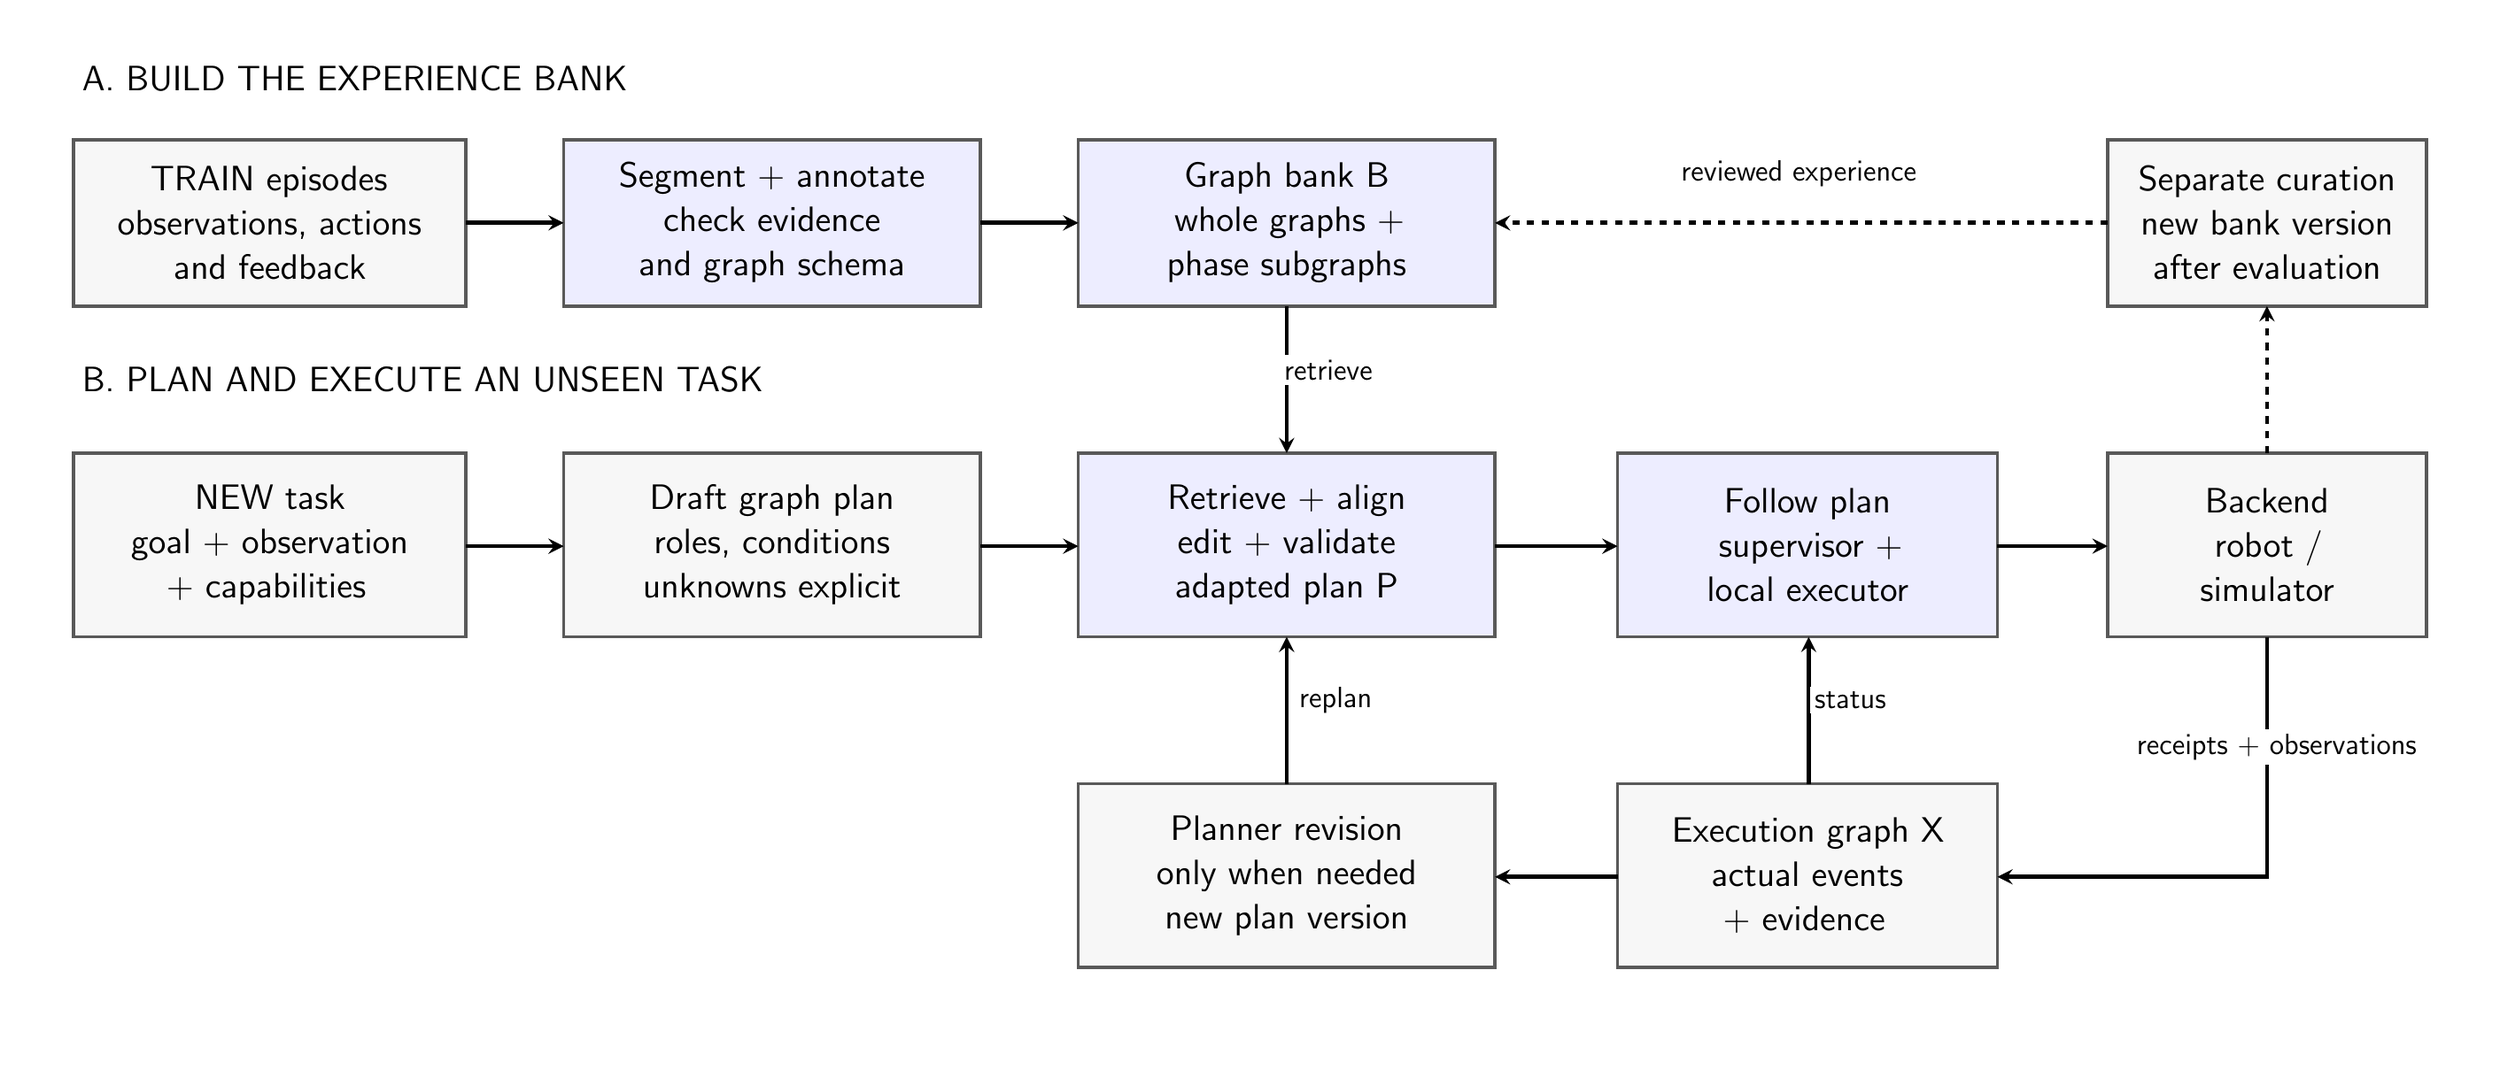
\begin{tikzpicture}[x=1pt,y=1pt,>=stealth]
\path[use as bounding box] (0,0) rectangle (1000,420);
\node[draw=black!65,fill=black!3,line width=1.3pt,minimum width=160pt,minimum height=68pt,text width=148pt,inner sep=4pt,align=center,font=\sffamily\fontsize{14}{18}\selectfont] (episodes) at (100.0,339.0) {TRAIN episodes\\observations, actions\\and feedback};
\node[draw=black!65,fill=blue!7,line width=1.3pt,minimum width=170pt,minimum height=68pt,text width=158pt,inner sep=4pt,align=center,font=\sffamily\fontsize{14}{18}\selectfont] (annotate) at (305.0,339.0) {Segment + annotate\\check evidence\\and graph schema};
\node[draw=black!65,fill=blue!7,line width=1.3pt,minimum width=170pt,minimum height=68pt,text width=158pt,inner sep=4pt,align=center,font=\sffamily\fontsize{14}{18}\selectfont] (bank) at (515.0,339.0) {Graph bank B\\whole graphs +\\phase subgraphs};
\node[draw=black!65,fill=black!3,line width=1.3pt,minimum width=160pt,minimum height=75pt,text width=148pt,inner sep=4pt,align=center,font=\sffamily\fontsize{14}{18}\selectfont] (input) at (100.0,207.5) {NEW task\\goal + observation\\+ capabilities};
\node[draw=black!65,fill=black!3,line width=1.3pt,minimum width=170pt,minimum height=75pt,text width=158pt,inner sep=4pt,align=center,font=\sffamily\fontsize{14}{18}\selectfont] (draft) at (305.0,207.5) {Draft graph plan\\roles, conditions\\unknowns explicit};
\node[draw=black!65,fill=blue!7,line width=1.3pt,minimum width=170pt,minimum height=75pt,text width=158pt,inner sep=4pt,align=center,font=\sffamily\fontsize{14}{18}\selectfont] (adapt) at (515.0,207.5) {Retrieve + align\\edit + validate\\adapted plan P};
\node[draw=black!65,fill=blue!7,line width=1.3pt,minimum width=155pt,minimum height=75pt,text width=143pt,inner sep=4pt,align=center,font=\sffamily\fontsize{14}{18}\selectfont] (follow) at (727.5,207.5) {Follow plan\\supervisor +\\local executor};
\node[draw=black!65,fill=black!3,line width=1.3pt,minimum width=130pt,minimum height=75pt,text width=118pt,inner sep=4pt,align=center,font=\sffamily\fontsize{14}{18}\selectfont] (world) at (915.0,207.5) {Backend\\robot /\\simulator};
\node[draw=black!65,fill=black!3,line width=1.3pt,minimum width=155pt,minimum height=75pt,text width=143pt,inner sep=4pt,align=center,font=\sffamily\fontsize{14}{18}\selectfont] (history) at (727.5,72.5) {Execution graph X\\actual events\\+ evidence};
\node[draw=black!65,fill=black!3,line width=1.3pt,minimum width=170pt,minimum height=75pt,text width=158pt,inner sep=4pt,align=center,font=\sffamily\fontsize{14}{18}\selectfont] (revise) at (515.0,72.5) {Planner revision\\only when needed\\new plan version};
\node[draw=black!65,fill=black!3,line width=1.3pt,minimum width=130pt,minimum height=68pt,text width=118pt,inner sep=4pt,align=center,font=\sffamily\fontsize{14}{18}\selectfont] (curate) at (915.0,339.0) {Separate curation\\new bank version\\after evaluation};
\draw[->,line width=1.7pt] (180,339) -- (220,339);
\draw[->,line width=1.7pt] (390,339) -- (430,339);
\draw[->,line width=1.7pt] (180,207) -- (220,207);
\draw[->,line width=1.7pt] (390,207) -- (430,207);
\draw[->,line width=1.7pt] (515,305) -- (515,245);
\node[fill=white,inner sep=2pt,font=\sffamily\fontsize{12}{14}\selectfont] at (532,279) {retrieve};
\draw[->,line width=1.7pt] (600,207) -- (650,207);
\draw[->,line width=1.7pt] (805,207) -- (850,207);
\draw[->,line width=1.7pt] (915,170) -- (915,72) -- (805,72);
\node[fill=white,inner sep=2pt,font=\sffamily\fontsize{12}{14}\selectfont] at (919,125) {receipts + observations};
\draw[->,line width=1.7pt] (650,72) -- (600,72);
\draw[->,line width=1.7pt] (515,110) -- (515,170);
\node[fill=white,inner sep=2pt,font=\sffamily\fontsize{12}{14}\selectfont] at (535,144) {replan};
\draw[->,line width=1.7pt] (728,110) -- (728,170);
\node[fill=white,inner sep=2pt,font=\sffamily\fontsize{12}{14}\selectfont] at (745,144) {status};
\draw[->,line width=1.7pt,dashed] (915,245) -- (915,305);
\draw[->,line width=1.7pt,dashed] (850,339) -- (600,339);
\node[fill=white,inner sep=2pt,font=\sffamily\fontsize{12}{14}\selectfont] at (724,359) {reviewed experience};
\node[anchor=base west,font=\sffamily\fontsize{15}{18}\selectfont] at (20,393) {A. BUILD THE EXPERIENCE BANK};
\node[anchor=base west,font=\sffamily\fontsize{15}{18}\selectfont] at (20,270) {B. PLAN AND EXECUTE AN UNSEEN TASK};
\end{tikzpicture}}
}
\caption{Proposed RoboRAG workflow. Training episodes are segmented and checked to form a versioned bank $\mathcal{B}$ of experience graphs $G$. A new goal, current observation and backend capabilities produce a draft plan $P$. Retrieved graphs or subgraphs supply phase structure, conditions and recovery evidence; alignment and validation produce an adapted plan. A supervisor follows approved phases through a local executor, while the planner handles structural revisions. Actual receipts and observations extend the execution graph $X$. The three graphs share a schema, but history, intent and observed execution retain distinct status. The training bank stays fixed during held-out evaluation; the dashed return path is used only by a separately evaluated curation process. This is a method diagram, not an experimental result.}
\label{fig:overview}
\end{figure*}

% END figures/01-overview.tex

% BEGIN sections/02-related.tex
\section{Related Work}
\label{sec:related}

\paragraph{Retrieval units and memory organization.}
Retrieval-augmented generation conditions a language model on an external information store~\cite{rag2020}. The contents and retrieval unit of that store matter as much as the search algorithm. G-Retriever retrieves connected portions of textual graphs for question answering~\cite{gretriever2024}. Its formulation illustrates how retrieval can preserve relations that independent text chunks omit. For manipulation, the corresponding design question is which parts of an interaction should remain connected: a prerequisite, an attempted action, its observed outcome, and a subsequent correction may jointly explain when an experience is useful. RoboRAG therefore treats the graph bank as part of the method. It stores episode graphs and indexes phase-centered subgraphs with evidence references, capability requirements, and versions. Retrieval must select experience that is applicable to the current decision, while retaining the information needed to assess that applicability.

\paragraph{Experience and in-context robot learning.}
RoboICL distinguishes demonstration context from the robot's accumulated interaction memory. Both use observation, action, receipt, and subsequent observation records; anchored memory retains selected earlier interactions~\cite{roboicl2026}. MemER learns to select task-relevant historical keyframes and uses them to produce instructions for a lower-level policy~\cite{memer2026}. These approaches motivate retaining useful history within a limited context budget. Memory Transfer Planning (MTP) is especially relevant to experience reuse across tasks: it stores successful planner code, retrieves examples through instruction similarity, adapts them to the target environment, and uses the adapted examples when replanning after failure~\cite{mtp2025}. RoboRAG examines a different retrieval unit: a phase together with its conditions, feedback, dependencies, and recovery links. Its bank includes observed failed attempts as well as successful continuations, allowing a query to distinguish experiences that share a goal but require different next actions.

\paragraph{Scene graphs, procedural graphs, and task graphs.}
These graph families encode different information. EmbodiedRAG retrieves task-relevant subgraphs from a changing three-dimensional scene representation~\cite{embodiedrag2024}. SafeMem accumulates objects and their relations in a semantic graph and uses this memory to assess action risks~\cite{safemem2026}. Such representations describe the environment. In RoboRAG, a node instead denotes an interaction-phase instance. Object relations appear as conditions or observations attached to that instance; edges describe temporal order, dependencies, conditional transitions, or recovery. This distinction makes explicit whether a record describes what exists, what was attempted, or what should happen next.

Procedural and task graphs are closer precedents. HP-KG constructs a hierarchy of tasks, steps, and actions with an automated multi-agent pipeline. It retrieves procedure nodes and associated subgraphs, then converts them into text for language-model planning~\cite{hpkg2025}. Neural Task Graphs infer a compositional graph from a demonstration and execute it by locating the current node and choosing transitions from visual observations~\cite{ntg2019}. RoboRAG's proposed distinction is the use of recorded phase outcomes and their evidence throughout graph construction, retrieval, adaptation, and execution monitoring. Temporal order alone does not establish a prerequisite or a recovery rule; the annotation procedure must preserve that distinction when converting an episode into reusable experience.

\paragraph{Grounded planning and delegated execution.}
SayCan combines language-model task reasoning with skill affordances~\cite{saycan2022}. Inner Monologue feeds environmental observations and success feedback into subsequent planning~\cite{innermonologue2022}. Code as Policies expresses robot behavior through programs that call perception and control APIs, including feedback loops~\cite{codepolicies2022}. GAVEL provides a particularly close execution comparison: a graph world model validates candidate plans, repairs errors implied by its action semantics, and returns unresolved violations to the language model~\cite{gavel2026}. These methods provide foundations for hierarchical execution and selective language-model invocation. RoboRAG assigns plan construction and substantial revision to a high-level planner, routine phase supervision to a smaller model, and bounded motion execution to local controllers. The question is whether retrieved phase evidence improves decisions at these interfaces, including when to continue, acquire another observation, repair a local plan, or request high-level replanning.

\paragraph{Research position.}
The proposed contribution is a shared representation linking episode annotation, graph-bank retrieval, task-conditioned adaptation, and observed execution. Its evaluation should compare HP-KG-style procedural retrieval, MTP-style reuse and adaptation, graph-based verification such as GAVEL, and linearized versions of the same evidence, with compatible information and controller access. These comparisons test the value of preserving phase, feedback, and dependency relations across the full experience-to-action process.

% Chapter summary: Prior work establishes graph retrieval, procedural reuse, task-graph execution, and selective replanning. RoboRAG studies an evidence-grounded phase graph shared across annotation, retrieval/adaptation, and delegated execution; matched evidence and controller comparisons must establish its value.

% END sections/02-related.tex

% BEGIN sections/03-formulation.tex
\section{Problem Formulation}
\label{sec:formulation}

We consider manipulation tasks specified by a goal $g$, an initial observation $o_0$, and a backend capability description $c$. The latter lists available observations, executable skills, argument types, and operating constraints. At decision step $t$, the system observes history $h_t=(o_0,a_0,f_0,\ldots,o_t)$, where $a_i$ is a skill request and $f_i$ its execution feedback. Observations and feedback may be incomplete. The task is to construct and follow a plan using this history and a bank of prior interaction graphs. Unseen tasks use supported skills in new task structures or object configurations. Section~\ref{sec:experiments} defines this novelty relative to the experimental bank and tuning data.

\paragraph{A shared graph schema.}
An interaction graph is $G=(V,E,A)$, with phase-instance nodes $V$, typed edges $E$, and an attribute map $A$. A phase is an interval of interaction organized around a local subgoal and a completion condition. Its node records the phase role, object-role bindings, an observed or symbolic interval, preconditions, intended effect, skill reference, feedback, and provenance. Object relations are predicates attached to nodes, rather than a second class of graph vertices. A node's intended effect is distinct from evidence that the effect occurred.

We use this schema for three different records: a historical experience graph $G$, a prospective plan $P_t$, and the current execution graph $X_t$. Historical nodes summarize recorded attempts, including failures. Plan nodes specify intended attempts and their conditions. Execution nodes record attempts made in the current episode. Thus, generating a plan node never establishes its completion in $X_t$.

\paragraph{Order, dependencies, and branches.}
A precedence edge constrains the order of two activated phases. A dependency edge names a prerequisite predicate that its source phase produces or verifies and its target requires. Such a relation is an annotation or a planning requirement; temporal order alone does not establish causation. A conditional transition enables a successor when its source reaches a terminal execution status and its guard is verified. A terminal receipt can activate an observation phase while the intended effect remains unknown. Later manipulation still requires verified prerequisites. A recovery link associates a failed attempt with a remedial phase and carries an activation guard. Precedence edges do not activate phases. When branches are alternatives, only the selected branch contributes ordering constraints.

Let $\operatorname{ver}(q,h_t)\in\{1,0,?\}$ denote whether available evidence verifies predicate $q$, refutes it, or leaves it unresolved. A node $v$ is ready when
\begin{equation}
\begin{split}
\operatorname{ready}(v,h_t)={}&
\operatorname{pre}(v,h_t)\ \land\ \operatorname{dep}(v,h_t)\\
&\land\ \operatorname{activate}(v,h_t)\ \land\ \operatorname{order}(v,X_t).
\end{split}
\label{eq:readiness}
\end{equation}
Here, $\operatorname{pre}$ requires verified preconditions, $\operatorname{dep}$ requires all mandatory prerequisite predicates, and $\operatorname{activate}$ holds for a designated entry node or at least one fired incoming transition or recovery link. Alternative incoming branches therefore use OR; mandatory dependencies use AND. The order term enforces precedence within activated branches. Concurrent ready nodes must also satisfy backend resource constraints. Unknown conditions do not count as true: they can trigger observation or planning revision. Completion likewise requires observed evidence for the node's completion predicate. A model's declaration of success is insufficient.

\paragraph{Time, revision, and the graph bank.}
Temporal structure includes observed intervals and precedence constraints, rather than only a list of phase labels. Dynamic structure means that annotation, new feedback, or plan revision can change attributes and topology. Versions retain node identities and provenance, with explicit lineage for splits or replacements. A plan may contain bounded retry logic; execution unrolls each attempt into a fresh event node. Consequently, realized temporal edges point forward in time even when a plan revisits a phase role.

The versioned RAG bank $\mathcal B^{(k)}$ stores historical graphs, their source episodes, and indexes for whole graphs and phase-centered subgraphs. Retrieval selects compatible experience; adaptation binds roles and revises parameters or topology using $h_t$ and $c$. The current execution graph remains separate from the frozen training bank during held-out evaluation. Cross-episode accumulation uses a separate chronological protocol.

\paragraph{Objective.}
The complete policy $\pi$ comprises planning, supervision, and local execution. It seeks evidence-verified task success under resource budgets:
\begin{equation}
\max_{\pi}\ \mathbb E\!\left[\mathbf 1\{\operatorname{ver}(g,h_T)=1\}\right],
\qquad \mathbf C(\pi)\preceq\mathbf b,
\label{eq:objective}
\end{equation}
where $\mathbf C$ records context consumption, model calls, execution time, and action attempts. Every dispatched skill must satisfy $c$. Phase estimates at deployment use observable history; reference annotations are reserved for construction and evaluation. Benchmark success oracles are evaluator-only and never supply control predicates.

% CHAPTER_SUMMARY: A versioned graph RAG bank connects historical experience G, prospective plans P_t, and observed execution X_t through one phase-instance schema. Typed edges distinguish temporal constraints, factual prerequisites, alternative guarded transitions, and recovery. Readiness combines mandatory prerequisites with alternative activation, while observed evidence determines completion. Unseen task composition remains bounded by backend skills; retrieval, adaptation, and hierarchical execution aim to improve verified success under cost budgets without evaluation leakage.

% END sections/03-formulation.tex
\section{Method}
\label{sec:method}

% BEGIN sections/04a-construction.tex
\subsection{Constructing a Bank of Interaction Graphs}
\label{sec:construction}

An experience should explain both what the robot attempted and what its feedback justified doing next. We therefore construct graphs from recorded interactions before building retrieval indices. A graph node represents one interaction phase, such as approaching an object, attempting a grasp, inspecting the result, or placing an object. Objects are arguments of phase predicates, not another type of node. This choice makes the graph describe a decision process whose structure can be reused as a plan.

\paragraph{From recordings to phase intervals.}
The input episode $\tau$ contains a task description, timestamped observations, proposed and executed actions, and controller receipts. We first split source episodes into data partitions, then annotate each episode within its partition. Records retain their sensor, coordinate-frame, action-interface, and source versions. A missing measurement remains unavailable; for example, a commanded gripper closure does not supply measured contact or object retention.

The proposed annotation pipeline has three passes. First, it proposes boundaries at changes in commanded skill or target role, gripper events, execution rejection or interruption, and observable changes relevant to the task. Second, a constrained annotator groups these candidates into intervals and assigns phase labels from a declared vocabulary. Its input includes the surrounding images, action receipts, and candidate event descriptions. Each interval has one immediate objective and a consistent action or observation role. Free-space movement towards one target may span many controller steps; a failed grasp followed by a new inspection creates separate phases because both the objective and the required evidence change. Labels outside the vocabulary are returned for vocabulary revision rather than silently introduced.

Third, validation checks the proposed intervals against their evidence. If a change is only localized between two observations, its boundary is stored as a bracket $[b_i^{-},b_i^{+}]$. A nominal boundary supports indexing, while the stored bracket preserves timing uncertainty. Ambiguous neighboring phases can remain a combined interval until the evidence supports a split. A second annotation pass flags disagreements in phase identity, target association, or outcome. Human adjudication resolves selected disagreements in the training annotations, with the decision and supporting records retained. At deployment, the agent uses the available observation history to estimate its phase. Prefix replay during annotation checks whether a label is already supported at the time it would be used; otherwise that prefix is labeled uncertain.

\paragraph{A common node and evidence schema.}
For $G=(V,E,A)$, the attribute map $A$ assigns each node an identifier, phase label, semantic object-role bindings, interval, preconditions, intended effect, action or skill reference, evidence references, outcome, and provenance. For example, a grasp phase binds the roles \texttt{manipulated\_object} and \texttt{acting\_gripper}. Its intended effect is \texttt{held(object, gripper)}. Whether that effect occurred is a separate field supported by observation references. A place phase uses the same object role and adds \texttt{destination}; its completion requires evidence about the object relative to that destination.

Predicates have typed arguments and a three-valued evidence state, $\operatorname{ver}(p,h_t)\in\{1,0,?\}$, as defined in Sec.~\ref{sec:formulation}.
Each evaluation names its observation or receipt, evaluation procedure, timestamp, and validity conditions. A visual interpretation is marked as estimated, while an execution receipt establishes only the controller facts it reports. Unresolved contradictions produce \(\mathsf{unknown}\). An annotator's confidence is stored separately from predicate truth and is not treated as a calibrated probability. These fields let a model read why a phase succeeded or failed without confusing a requested action with its outcome.

The same schema also represents prospective nodes in $P_t$ and realized nodes in $X_t$. A prospective node specifies a completion predicate and the evidence needed to check it; it has no observed completion value. When executed, it creates a new event node linked to its plan-node identifier and plan version. Historical evidence stays attached to its source episode when the node is retrieved. It cannot certify a predicate in the current scene.

\paragraph{Encoding transitions and recovery.}
Edge records instantiate the readiness rule in Eq.~\ref{eq:readiness}. Each transition or recovery edge records its guard and supporting evidence; each dependency names the required predicate. Mutually exclusive outgoing alternatives share a branch identifier, and at most one can be selected.

Consider putting a bottle in a bin. The first grasp attempt ends with images showing the bottle still on the table after the gripper moves away. Its effect \texttt{held} is false under the declared visual check. A recovery link guarded by that failed effect activates re-observation, which establishes a fresh bottle reference. A second grasp depends on that reference. Once retention is verified, the plan can activate placement and then check that the bottle is inside the bin. The recovery link preserves the relation between the first failed attempt and re-observation; the successful second attempt does not overwrite the failure. If retention is occluded, the graph takes an inspection step instead of assigning success. A retry template specifies a finite attempt budget. Execution unrolls it into distinct event nodes, so repeated attempts preserve their individual actions, feedback, and costs.

\paragraph{Validation and agent-readable serialization.}
The stored representation uses a versioned JSON schema and a predicate dictionary. A validator checks role types, referenced evidence, interval consistency, edge endpoints, branch identifiers, and finite retry budgets. It also checks that a claimed observed effect has a valid evidence reference and that dependencies can be satisfied along an eligible route. Prospective geometry may remain unresolved, but an executable action must name its current grounded target and required capability.

For model input, a deterministic renderer presents each selected node as a short record: role and objective, entry condition, permitted skill, completion evidence, observed outcome if any, and eligible successors. A worked record shows how \texttt{unknown} differs from failure. Both the compact description and the structured record come from the same fields; free-text summaries cannot change the edge guards.

\paragraph{Whole-graph and subgraph indices.}
Each whole graph is indexed by task relation, role types, phase sequence, available capabilities, and entry-state features. A second index stores phase-centered subgraphs. A seed contains a phase and its adjacent transitions; its closure adds the dependency and recovery-trigger records needed to interpret those transitions. Thus, retrieving a regrasp preserves the preceding failure and the observation that made a new attempt reasonable. Each index entry points to immutable graph, node, and media identifiers. Search descriptors represent conditions at the subgraph entry, while the payload retains later outcomes for comparison and adaptation. This separates a queryable situation from the result of the historical response.

\paragraph{Versioned updates.}
Annotation corrections create a new graph version with stable surviving node identifiers and explicit replacements for split or merged phases. Only affected descriptors, subgraph closures, and index entries are rebuilt. During execution, completed or interrupted events extend $X_t$; plan patches create new versions of $P_t$. Neither operation modifies the frozen training bank used in the main evaluation. Cross-episode accumulation instead runs an offline admission step that validates evidence, checks partitions, removes duplicates, and publishes a new bank snapshot. The resulting bank preserves both useful successful procedures and the conditions that motivated recovery.

% CHAPTER_SUMMARY: The proposed annotation pipeline converts source episodes into evidence-linked interaction-phase graphs. Typed conditions, branch semantics, recovery links, stable identities, and validated serialization connect historical experience to prospective plans without treating intended effects as observed outcomes. Whole-graph and dependency-complete subgraph indices preserve the context needed to adapt failures and recoveries; bank updates remain versioned and separate from current-episode execution.

% END sections/04a-construction.tex

% BEGIN figures/02-graph-semantics.tex
\begin{figure*}[t]
\centering
\RoboRAGFigure{02-graph-semantics-nature.png}{%
\resizebox{\textwidth}{!}{%
\begin{tikzpicture}[x=1pt,y=1pt,>=stealth]
\path[use as bounding box] (0,0) rectangle (1000,420);
\node[draw=black!65,fill=black!3,line width=1.3pt,minimum width=165pt,minimum height=80pt,text width=153pt,inner sep=4pt,align=center,font=\sffamily\fontsize{14}{18}\selectfont] (g1) at (102.5,290.0) {v1: grasp attempt\\[0, 2] s\\outcome: failed};
\node[draw=black!65,fill=black!3,line width=1.3pt,minimum width=165pt,minimum height=80pt,text width=153pt,inner sep=4pt,align=center,font=\sffamily\fontsize{14}{18}\selectfont] (observe) at (322.5,290.0) {v2: reobserve\\[2, 3] s\\new object pose};
\node[draw=black!65,fill=blue!7,line width=1.3pt,minimum width=165pt,minimum height=80pt,text width=153pt,inner sep=4pt,align=center,font=\sffamily\fontsize{14}{18}\selectfont] (g2) at (542.5,290.0) {v3: grasp attempt\\[3, 5] s\\holding verified};
\node[draw=black!65,fill=black!3,line width=1.3pt,minimum width=205pt,minimum height=80pt,text width=193pt,inner sep=4pt,align=center,font=\sffamily\fontsize{14}{18}\selectfont] (place) at (862.5,290.0) {v4: place\\[5, 7] s\\placement verified};
\node[draw=black!65,fill=black!3,line width=1.3pt,minimum width=600pt,minimum height=155pt,text width=588pt,inner sep=4pt,align=center,font=\sffamily\fontsize{15}{18}\selectfont] (record) at (320.0,92.5) {Example record for v1\\role: grasp(item)     binding: item = cup\_7\\precondition: reachable(item)\\intended effect: holding(item)\\observed outcome: failed; evidence = frames\_18\_21\\source: TRAIN episode\_12; interval = [0, 2] s};
\node[draw=black!65,fill=black!3,line width=1.3pt,minimum width=285pt,minimum height=155pt,text width=273pt,inner sep=4pt,align=center,font=\sffamily\fontsize{15}{18}\selectfont] (guard) at (822.5,92.5) {Ready to start a phase?\\An eligible branch is selected (OR)\\AND every prerequisite is true\\AND resources are available\\Unknown condition: observe first\\Requested effect is not completion};
\draw[->,line width=1.7pt] (185,290) -- (240,290);
\draw[->,line width=1.7pt] (405,290) -- (460,290);
\draw[->,line width=1.7pt] (625,290) -- (760,290);
\node[fill=white,inner sep=2pt,font=\sffamily\fontsize{12}{14}\selectfont] at (665,309) {temporal};
\draw[->,line width=1.7pt,dashed] (103,330) -- (103,375) -- (322,375) -- (322,330);
\node[fill=white,inner sep=2pt,font=\sffamily\fontsize{12}{14}\selectfont] at (280,393) {recovery: failure to reobservation};
\draw[->,line width=1.7pt,dotted] (543,250) -- (543,215) -- (862,215) -- (862,250);
\node[fill=white,inner sep=2pt,font=\sffamily\fontsize{12}{14}\selectfont] at (701,203) {dependency: holding(item) = true};
\node[anchor=base west,font=\sffamily\fontsize{14}{18}\selectfont] at (20,408) {ILLUSTRATIVE OBSERVED GRAPH: FOUR DISTINCT PHASE INSTANCES};
\end{tikzpicture}}
}
\caption{An interaction graph records phase instances and the evidence connecting them. In this illustrative recorded episode, a grasp attempt fails; reobservation and a second attempt precede placement. Each box is a phase instance, not an object. Solid arrows show the observed temporal order. The dashed recovery link connects the failed attempt to reobservation; the second grasp uses the newly grounded target. The dotted dependency states that placement requires verified holding evidence from the second grasp. Alternative success and failure guards are transition choices (OR), whereas prerequisites must all hold (AND). The node record separates the requested effect from its observed outcome. A plan may contain bounded retry logic; recorded attempts have distinct IDs and times. Times and evidence IDs in this example illustrate the schema and are not measured experimental data.}
\label{fig:semantics}
\end{figure*}

% END figures/02-graph-semantics.tex

% BEGIN sections/04b-use.tex
\subsection{Retrieving, Adapting, and Following Interaction Graphs}
\label{sec:graph-use}

The second part of RoboRAG turns stored experience into a plan for the current task. A shared schema makes each retrieved phase interpretable as a conditional procedure: what it requires, what it attempts, what evidence would establish completion, and which continuation its outcome permits. The proposed execution hierarchy separates changes to this procedure from routine decisions within it.

\paragraph{An initial plan under the shared schema.}
The planner receives the goal $g$, current observations, capability description $c$, and a compact graph specification. The specification defines every field and edge type, provides one annotated example, and pairs each skill with its argument schema and observable completion conditions. The planner generates a structured record. Each node contains a symbolic phase role, typed object variables, preconditions, a skill reference, intended effects, and an evidence requirement. A short explanation accompanies each node for inspection, while execution reads the structured fields. Object variables must bind to observable entities or remain explicitly unresolved.

The first output is a provisional graph $P_t^{-}$. It identifies possible phases and missing information before retrieval. A schema checker returns errors at specific node or edge identifiers; the planner receives these errors for a bounded correction pass. Missing geometry can remain symbolic until perception supplies it. An unresolved object identity requires an observation phase or clarification through the task interface. Dispatch requires grounded coordinates and bindings. This provisional graph guides search without fixing the final phase sequence.

\paragraph{Searching graphs and local experience.}
A retrieval query combines the goal, estimated current phase, observed predicates, unresolved prerequisites, and available skills:
\begin{equation}
q_t=(g,\hat z_t,\mathcal F_t,\mathcal U_t,c,P_t^{-}),
\label{eq:graph-query}
\end{equation}
where $\hat z_t$ can be unknown, $\mathcal F_t$ contains evidence-backed current facts, and $\mathcal U_t$ contains missing conditions. The phase estimate uses $h_t$, not reference segmentation labels. At episode start, the goal and provisional graph dominate the query. After a failed attempt, its phase, feedback, and unmet effect specify the local search context.

Two indexes supply candidates under a shared retrieval budget. Whole-graph search finds procedures with related goals and compatible phase structure. Phase-centered search finds smaller patterns around an unmet prerequisite, failure, or intended effect. A candidate retains its boundary conditions and supporting evidence. If its dependency closure exceeds the budget, search chooses another complete candidate or returns no compatible evidence. Capability filtering rejects procedures whose required skills have neither a supported implementation nor an explicitly declared replacement. Source trajectories provide context, while current observations determine execution geometry.

A reranker searches for a type-consistent role mapping $M$ and a partial node alignment between a candidate $H$ and the provisional plan. Its score is
\begin{equation}
\begin{split}
s(H,q_t)=\max_M\{&w_g s_g+w_r s_r(M)+w_f s_f(M)\\
                &+w_e s_e(M)+w_o s_o(M)-\lambda d(M)\},
\end{split}
\label{eq:alignment-score}
\end{equation}
where the terms measure goal similarity, role compatibility, condition compatibility, preservation of typed edges, and relevance of recorded outcomes. The penalty $d$ estimates required edits and context cost. Role compatibility includes functional and physical constraints: a movable item and an articulated receptacle cannot be interchanged because their names are similar. Conditions receive separate treatment when already verified, achievable through a supported prerequisite, unresolved, or contradicted. Unresolved conditions incur uncertainty; contradictions reject the alignment unless an explicit action can change them. Edge matching rewards compatible local structure without requiring the target to duplicate a complete source graph. Weights, retrieval count, and acceptance thresholds are selected on development tasks and fixed for held-out evaluation.

\paragraph{Adapting a retrieved procedure.}
The planner receives a small set of scored candidates, alignment proposals, and their evidence references. It returns a graph plus an explicit edit list. It can rebind object roles, revise skill parameters within declared bounds, or insert a prerequisite. It can also replace an unavailable phase with a supported sequence that has the required effect, or add a recovery branch with an activation condition and retry limit. Edits can combine compatible subgraphs. Each copied or changed node retains source provenance, and newly proposed nodes are labeled as such.

Parameter adaptation is separate from mandatory geometric grounding. All executable plans use current object poses and the same feasibility checks. Where a skill exposes these choices, the planner can additionally change the approach direction in the object's reference frame and the precontact clearance distance within the skill's admissible bounds. These edits preserve the phase role and graph topology. Live-pose grounding transforms the approved parameters into current execution coordinates; it is required even when the planner retains the source parameter choices. Infeasible retained parameters are rejected before dispatch.

Figure~\ref{fig:adaptation} illustrates a held-out composition: placing a cup into a closed drawer. Transfer experience provides grasp, move, and place phases. Drawer-opening experience supplies a missing prerequisite. Adaptation binds the item role to the current cup, inserts opening and handle release before the cup grasp for a single-gripper robot, and grounds motion parameters from the current scene. A recorded failed grasp can supply a branch that observes the scene again and retries the grasp. Its retry count and admissible parameter adjustments are specified before execution.

\paragraph{Checking the plan before use.}
Validation checks schema types, object bindings, skill support, predicate references, resource conflicts, and graph structure under the readiness semantics of Sec.~\ref{sec:formulation}. Every intended terminal goal must have a supported path from an entry node. All mandatory dependency predicates need an evidence source or a reachable producing phase. The validator requires exclusive branch guards or a declared priority when alternatives can fire together. Activated dependencies and temporal constraints must admit an execution order, and unresolved preconditions block dispatch. Retry links require a finite budget and generate fresh execution instances.

A successful structural check does not predict physical success. It establishes that the procedure is interpretable and that its next authorized step can be checked against current evidence. Validation errors return to the planner as a bounded repair request. If no compatible candidate passes retrieval thresholds, planning continues from $g$, $h_t$, and $c$ using the same schema. If adaptation fails validation, the planner can discard the retrieved procedure and construct a fresh graph. Exhausted repair budgets or an unsupported task produce an explicit unresolved outcome rather than a forced action.

\paragraph{Delegated plan following.}
The hierarchy has three roles. The high-level planner constructs or structurally revises $P_t$; Astra is a candidate implementation. A lower-cost supervisor, for example Luna, reads the active phase neighborhood, recent feedback, and evidence references. It can select ready phases, choose an already approved conditional branch, request a listed observation, and invoke an approved recovery step. It cannot add nodes, change object identities, relax completion conditions, or extend a recovery budget. A deterministic execution gateway validates each request and sends its skill and bounded arguments to the backend's local controller. Servo control remains local.

Parameter updates have a narrow authority boundary. A supervisor may request re-estimation of a pose through an approved perception skill, and the grounding module may refresh geometry within the active node's workspace and tolerance. It preserves the approved approach direction and clearance choices; changing either requires a versioned planner edit. A changed target role, unsupported grasp strategy, violated resource constraint, or adjustment outside those bounds also requires planner revision. The planner handles conflicting evidence, repeated unresolved conditions, and exhausted recovery branches. Routine successful receipts remain with the supervisor.

\paragraph{Evidence, receipts, and revisions.}
Each dispatch carries the plan version, node identifier, attempt identifier, and an idempotent request identifier. The gateway rejects stale versions and unauthorized arguments. An accepted request is pending until its terminal receipt arrives; acknowledgment is not phase completion. A receipt-guarded observation transition may then activate a verification phase while the action's intended effect remains unknown. Task progress requires evidence for that effect, and subsequent manipulation remains blocked until its prerequisites hold. Predicate evaluators use allowed sensor observations or backend feedback and return evidence references with true, false, or unknown. A visual evaluator uses fixed acceptance rules checked on development data; unsupported or ambiguous judgments remain unknown. Benchmark success oracles are accessible only to the evaluator and never supply control predicates.

Every actual attempt appends an event to $X_t$, including failed and interrupted attempts. Recovery creates a new event linked to the failed event; it cannot overwrite that failure. Plan edits increment the version, preserve unchanged node identifiers, and record replacement lineage. Revisions activate only after outstanding requests finish or cancellation is confirmed, preventing a new plan from treating an unresolved action as absent. Evidence-dependent readiness is recomputed after each terminal event or relevant observation. Cached retrieval results are reconsidered when the active phase, condition signature, plan structure, or capability description changes.

\paragraph{Memory during execution.}
The current execution graph updates the context for subsequent queries and plan revisions. Bank admission follows the versioned update procedure in Sec.~\ref{sec:construction}; Sec.~\ref{sec:experiments} evaluates fixed-bank execution and cross-episode accumulation separately.

\paragraph{Execution procedure.}
The following procedure summarizes the planning and supervision loop; all budgets are declared before a run.
\begin{enumerate}
\item Construct and schema-check $P^{-}$ from $(g,h_0,c)$. Retrieve whole graphs and phase subgraphs, align candidates, and propose an edited plan.
\item Validate the plan. Repair within budget, fall back to planning under the same schema if retrieval is unsuitable, or stop with an unresolved outcome.
\item Evaluate active predicates from available evidence. If the goal is verified, finish; if required evidence is missing, take an authorized observation step or escalate.
\item Let the supervisor select a ready, resource-compatible phase or an approved recovery branch. The gateway checks version, authority, and arguments before dispatch.
\item Resolve the receipt, append the attempt and evidence to $X$, and update predicates. Continue the approved plan when its conditions hold.
\item On a structural mismatch or exhausted local recovery, retrieve again and ask the planner for a versioned revision. Stop when the task, action, observation, or revision budget is exhausted.
\end{enumerate}

% CHAPTER_SUMMARY: A planner drafts unseen-task graphs under the shared schema, retrieves whole procedures and local evidence, aligns roles/conditions/typed structure, and makes explicit parameter or structural edits. Mandatory live-pose grounding is common to every executable plan. A smaller supervisor follows approved phases and recovery branches, while a deterministic gateway enforces requests and local controllers execute skills; parameter choices and structural changes return to the planner. Receipt-backed evidence determines progress, revisions retain lineage, and failed attempts remain in X.

% END sections/04b-use.tex

% BEGIN figures/03-plan-adaptation.tex
\begin{figure*}[t]
\centering
\RoboRAGFigure{03-plan-adaptation-nature.png}{%
\resizebox{\textwidth}{!}{%
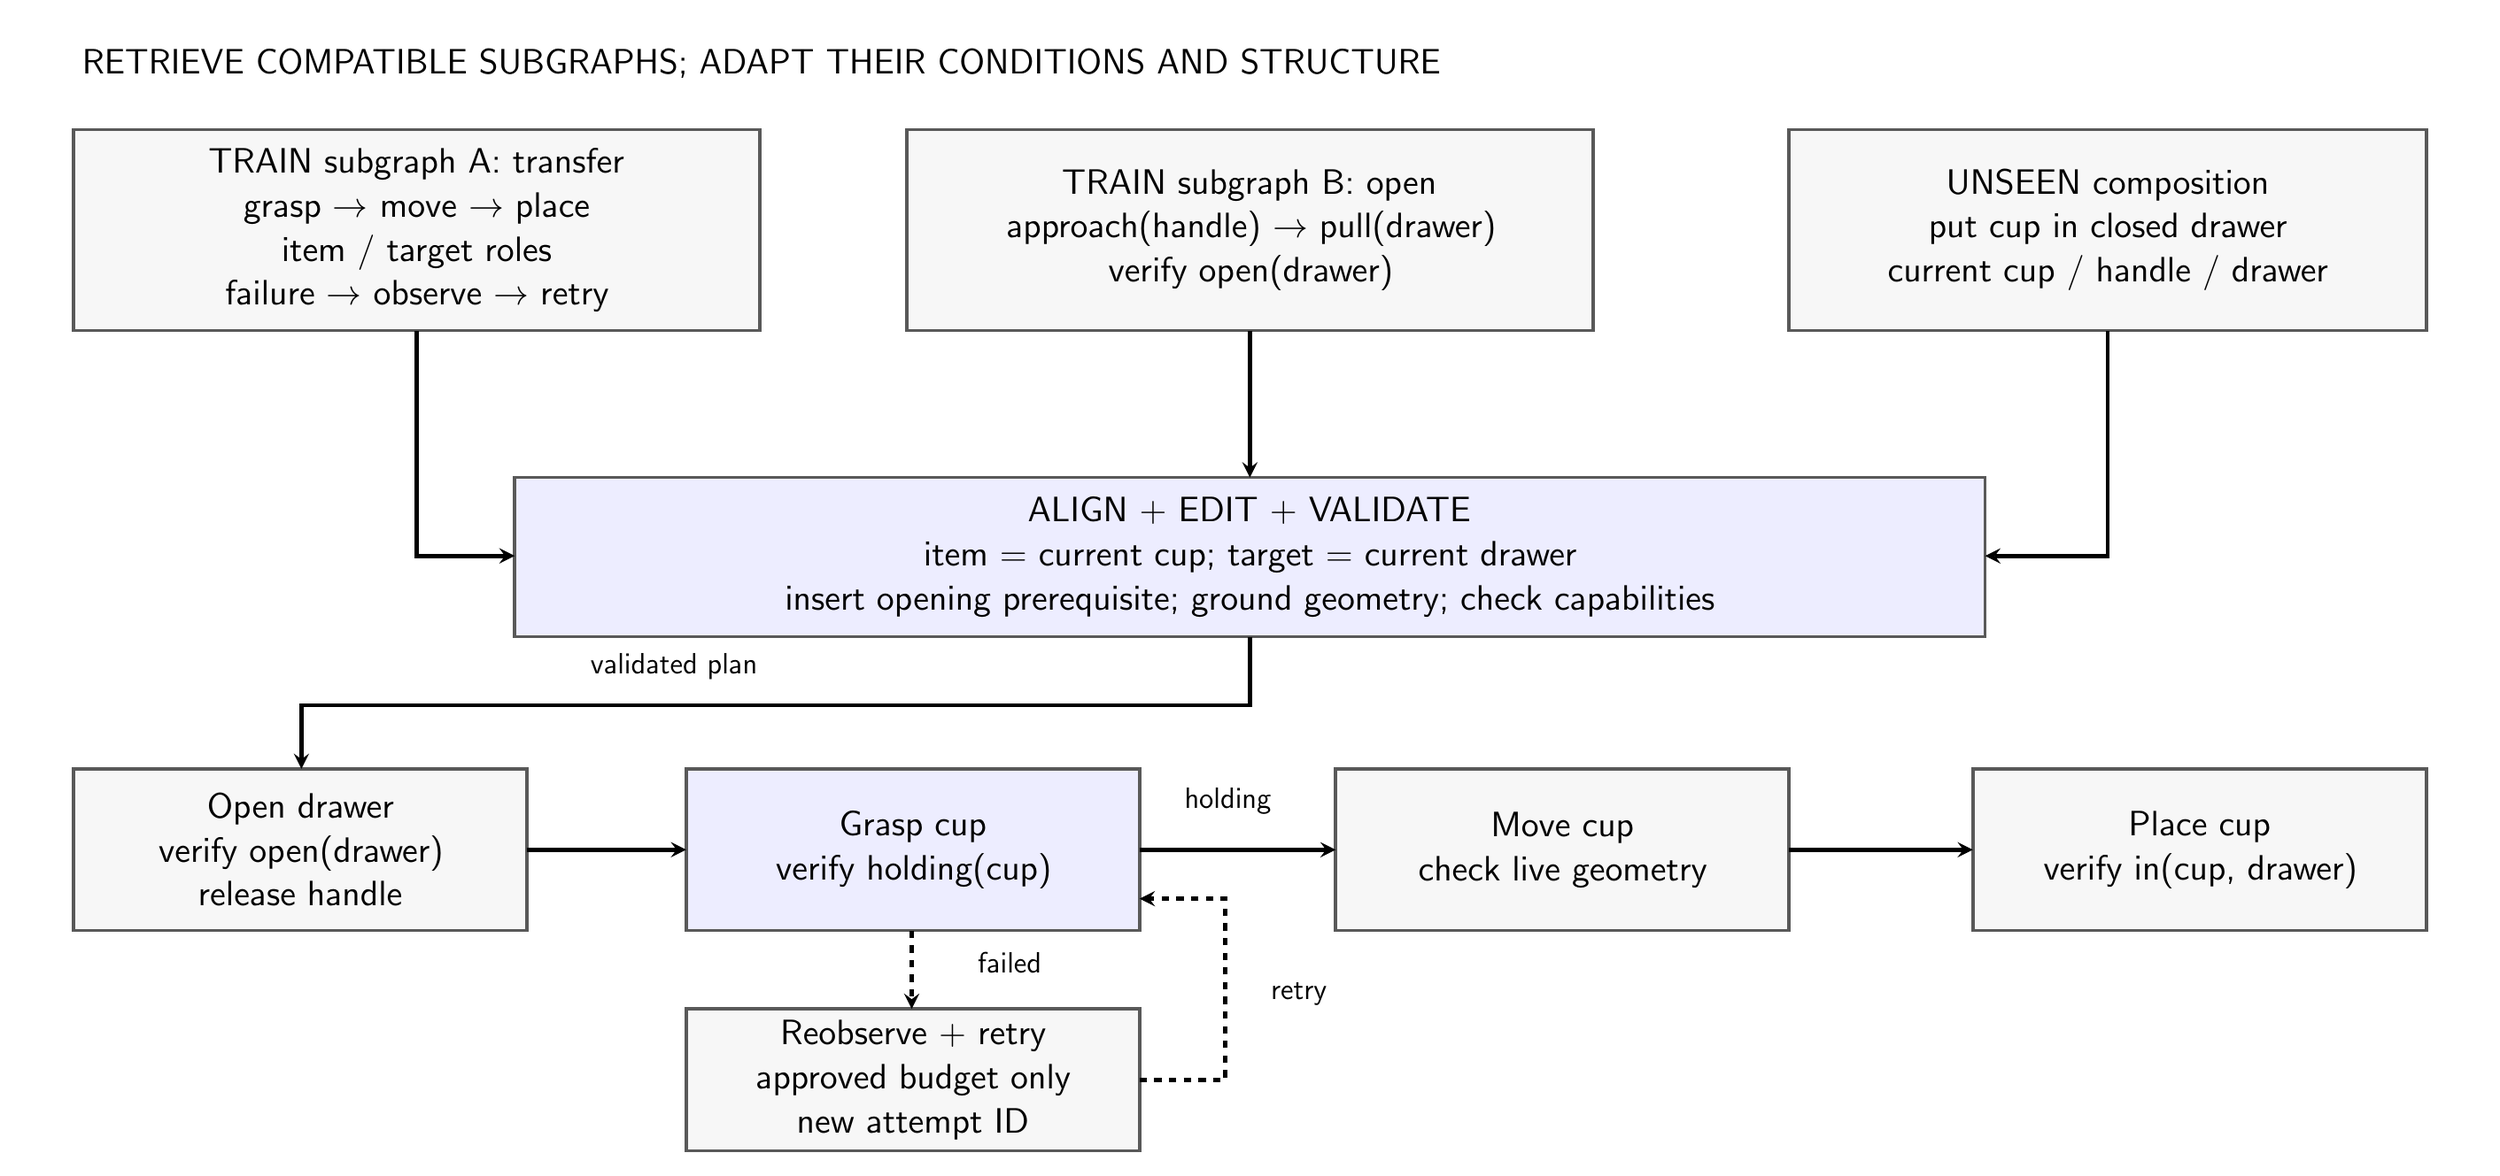
\begin{tikzpicture}[x=1pt,y=1pt,>=stealth]
\path[use as bounding box] (0,0) rectangle (1000,460);
\node[draw=black!65,fill=black!3,line width=1.3pt,minimum width=280pt,minimum height=82pt,text width=268pt,inner sep=4pt,align=center,font=\sffamily\fontsize{15}{18}\selectfont] (source1) at (160.0,376.0) {TRAIN subgraph A: transfer\\grasp $\rightarrow$ move $\rightarrow$ place\\item / target roles\\failure $\rightarrow$ observe $\rightarrow$ retry};
\node[draw=black!65,fill=black!3,line width=1.3pt,minimum width=280pt,minimum height=82pt,text width=268pt,inner sep=4pt,align=center,font=\sffamily\fontsize{15}{18}\selectfont] (source2) at (500.0,376.0) {TRAIN subgraph B: open\\approach(handle) $\rightarrow$ pull(drawer)\\verify open(drawer)};
\node[draw=black!65,fill=black!3,line width=1.3pt,minimum width=260pt,minimum height=82pt,text width=248pt,inner sep=4pt,align=center,font=\sffamily\fontsize{15}{18}\selectfont] (query) at (850.0,376.0) {UNSEEN composition\\put cup in closed drawer\\current cup / handle / drawer};
\node[draw=black!65,fill=blue!7,line width=1.3pt,minimum width=600pt,minimum height=65pt,text width=588pt,inner sep=4pt,align=center,font=\sffamily\fontsize{15}{18}\selectfont] (align) at (500.0,242.5) {ALIGN + EDIT + VALIDATE\\item = current cup; target = current drawer\\insert opening prerequisite; ground geometry; check capabilities};
\node[draw=black!65,fill=black!3,line width=1.3pt,minimum width=185pt,minimum height=66pt,text width=173pt,inner sep=4pt,align=center,font=\sffamily\fontsize{14}{18}\selectfont] (open) at (112.5,123.0) {Open drawer\\verify open(drawer)\\release handle};
\node[draw=black!65,fill=blue!7,line width=1.3pt,minimum width=185pt,minimum height=66pt,text width=173pt,inner sep=4pt,align=center,font=\sffamily\fontsize{14}{18}\selectfont] (grasp) at (362.5,123.0) {Grasp cup\\verify holding(cup)};
\node[draw=black!65,fill=black!3,line width=1.3pt,minimum width=185pt,minimum height=66pt,text width=173pt,inner sep=4pt,align=center,font=\sffamily\fontsize{14}{18}\selectfont] (move) at (627.5,123.0) {Move cup\\check live geometry};
\node[draw=black!65,fill=black!3,line width=1.3pt,minimum width=185pt,minimum height=66pt,text width=173pt,inner sep=4pt,align=center,font=\sffamily\fontsize{14}{18}\selectfont] (place) at (887.5,123.0) {Place cup\\verify in(cup, drawer)};
\node[draw=black!65,fill=black!3,line width=1.3pt,minimum width=185pt,minimum height=58pt,text width=173pt,inner sep=4pt,align=center,font=\sffamily\fontsize{14}{18}\selectfont] (retry) at (362.5,29.0) {Reobserve + retry\\approved budget only\\new attempt ID};
\draw[->,line width=1.7pt] (160,335) -- (160,243) -- (200,243);
\draw[->,line width=1.7pt] (500,335) -- (500,275);
\draw[->,line width=1.7pt] (850,335) -- (850,243) -- (800,243);
\draw[->,line width=1.7pt] (500,210) -- (500,182) -- (113,182) -- (113,156);
\node[fill=white,inner sep=2pt,font=\sffamily\fontsize{12}{14}\selectfont] at (265,198) {validated plan};
\draw[->,line width=1.7pt] (205,123) -- (270,123);
\draw[->,line width=1.7pt] (455,123) -- (535,123);
\node[fill=white,inner sep=2pt,font=\sffamily\fontsize{12}{14}\selectfont] at (491,143) {holding};
\draw[->,line width=1.7pt] (720,123) -- (795,123);
\draw[->,line width=1.7pt,dashed] (362,90) -- (362,58);
\node[fill=white,inner sep=2pt,font=\sffamily\fontsize{12}{14}\selectfont] at (402,77) {failed};
\draw[->,line width=1.7pt,dashed] (455,29) -- (490,29) -- (490,103) -- (455,103);
\node[fill=white,inner sep=2pt,font=\sffamily\fontsize{12}{14}\selectfont] at (520,64) {retry};
\node[anchor=base west,font=\sffamily\fontsize{14}{18}\selectfont] at (20,440) {RETRIEVE COMPATIBLE SUBGRAPHS; ADAPT THEIR CONDITIONS AND STRUCTURE};
\end{tikzpicture}}
}
\caption{Illustrative retrieval and adaptation for a new task: place a cup in a closed drawer. Two training subgraphs provide object transfer and drawer opening; the target composition is held out from the experience bank. Object roles are rebound to current observations, the open-drawer phase is inserted as a prerequisite, and current geometry supplies the action parameters. The adapted plan also incorporates an authorized recovery branch from historical failure evidence. The supervisor checks predicates and follows the approved branch; structural changes go to the planner. A failed grasp appends a failed event to $X$ and creates a distinct retry instance, rather than relabeling the failed action as successful. The example explains graph composition and revision; it makes no claim that this task has been implemented or solved.}
\label{fig:adaptation}
\end{figure*}

% END figures/03-plan-adaptation.tex

% BEGIN sections/05-system.tex
\section{System Framework}
\label{sec:system}

RoboRAG connects graph planning to robot execution through a common semantic contract. The contract describes what a backend can do, what its observations mean, and what evidence an action returns. We propose adapters for RoboDojo, LIBERO~\cite{libero2023}, and a real robot. This separation allows the same planner to inspect backend capabilities and revise a graph before dispatch. MCP supplies a standard interface for discovering and invoking tools~\cite{mcp2026}; the robot semantics remain defined by RoboRAG and implemented by each adapter.

\subsection{Capabilities, Observations, and Actions}

\paragraph{Capabilities.}
A versioned capability description identifies the robot, arms, controlled links, tool-center-point transforms, supported skills, sensors, coordinate frames, and units. It also declares motion limits, control periods, and available hold and stop operations. Each skill specifies input types, required observations, and possible outcomes. The adapter derives these declarations from its configuration and implemented functions. An unsupported capability produces a structured rejection that the planner can use to select another skill or revise the plan.

\paragraph{Observations.}
A snapshot carries an episode identifier, state sequence, camera capture times, calibration version, and state provenance. Fields distinguish measured, estimated, commanded, and unavailable values. For example, a commanded gripper width cannot establish object retention. Poses identify their reference frame, controlled link, orientation convention, and timestamp. Object estimates retain their sensor source and validity interval. Simulation steps, simulation time, and monotonic wall-clock time occupy separate fields. These distinctions let a graph condition refer to evidence with a defined meaning across adapters.

\paragraph{Actions.}
A motion request specifies an absolute target or bounded segment, its frame, the relevant plan version and phase authorization, required preconditions, and an expiry time. Gripper commands are explicit and separately authorized. The adapter checks state freshness, calibration, numerical validity, supported limits, and feasibility before dispatch. If a backend uses incremental commands, conversion uses one identified starting snapshot; later dispatch windows continue the converted targets. New geometry comes from current observations and the target backend. A retrieved graph contributes phase structure and conditions rather than source-platform coordinates.

\subsection{Execution Receipts and Local Control}

Each accepted request receives an execution identifier. Receipts distinguish acceptance, dispatch, confirmed execution, remaining commands, invalidated commands, and unknown outcomes. They record the executed prefix and the reason for termination. Motion completion establishes only the corresponding execution fact; a phase requiring successful grasp or placement still needs its specified observation evidence. The supervisor uses these receipts to update the execution history $X_t$ and decide whether the active plan $P_t$ can advance.

An episode and request identifier together provide deduplication. Repeating an identical request returns its existing execution record; reusing the identifier with different parameters is rejected. After a communication timeout, the client queries execution state instead of resubmitting motion. An uncertain outcome blocks further dispatch until the adapter reconciles the execution record and obtains the required state evidence. Plan patches must match the current version, so a delayed response cannot restore a cancelled segment.

Servo control, interpolation, tracking checks, and physical protection remain in the native backend. The adapter exposes their supported behavior, including the effect of pause, cancel, and stop on outstanding motion and gripper commands. A cancellation acknowledgment is distinct from evidence that a physical robot has stopped. Local protection must operate independently of language-model inference. We evaluate synchronous simulation and continuous physical execution separately, reporting measured wall-clock timing alongside nominal controller frequency.

Section~\ref{sec:evidence-analysis} describes the existing execution infrastructure and the implementation status of the proposed framework.

\subsection{Separating Interface Reuse from MCP Transport}

Figure~\ref{fig:platform} compares three modes within each backend. Mode A accesses the backend through a specific native driver. Mode B uses the common contract and adapter through direct calls. Mode C exposes that same contract and adapter through MCP. B versus A tests semantic normalization and application reuse; C versus B tests the incremental effects of protocol discovery and transport.

Differences in embodiment, sensing, contact dynamics, and available skills remain explicit in the adapters. Shared access can reduce integration work, while successful experience transfer depends on compatible graph conditions and adaptation to the receiving platform. Section~\ref{sec:experiments} specifies the controlled comparisons and measures porting effort, conformance, timing, and task performance per backend.

% CHAPTER_SUMMARY: A common capability, observation, action, and receipt contract connects graph planning to native execution. Provenance, frames, timing, authorization, and execution evidence preserve graph semantics across adapters. Native servo and protection functions retain local responsibility. Comparing native access, normalized direct access, and the same normalized interface through MCP isolates application reuse from protocol effects across proposed RoboDojo, LIBERO, and real-robot targets.

% END sections/05-system.tex

% BEGIN figures/04-platform-comparison.tex
\begin{figure*}[t]
\centering
\RoboRAGFigure{04-platform-comparison-nature.png}{%
\resizebox{\textwidth}{!}{%
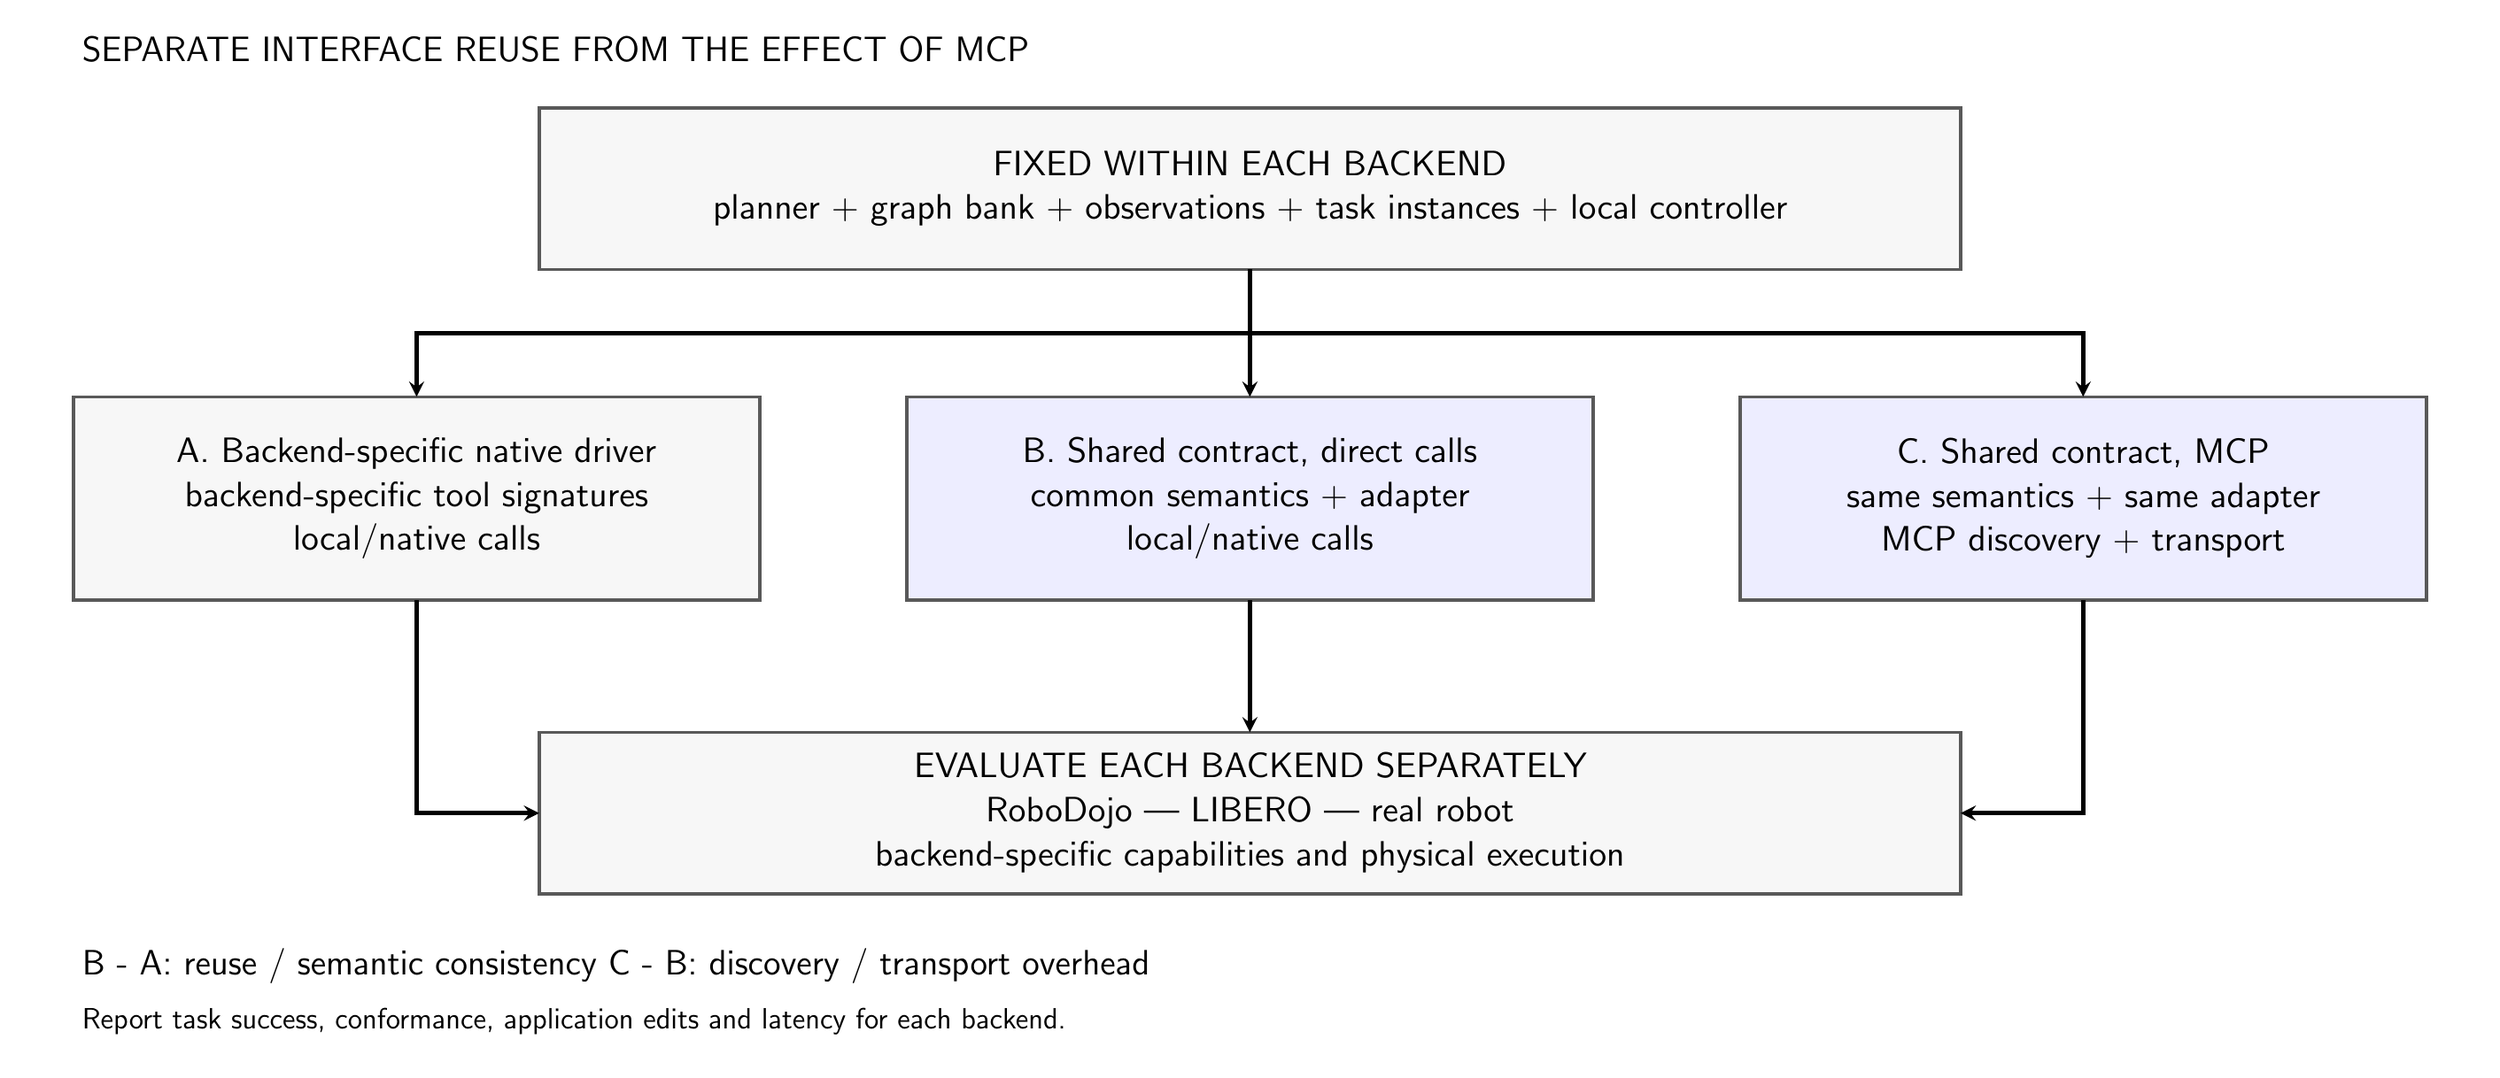
\begin{tikzpicture}[x=1pt,y=1pt,>=stealth]
\path[use as bounding box] (0,0) rectangle (1000,420);
\node[draw=black!65,fill=black!3,line width=1.3pt,minimum width=580pt,minimum height=66pt,text width=568pt,inner sep=4pt,align=center,font=\sffamily\fontsize{15}{18}\selectfont] (shared) at (500.0,353.0) {FIXED WITHIN EACH BACKEND\\planner + graph bank + observations + task instances + local controller};
\node[draw=black!65,fill=black!3,line width=1.3pt,minimum width=280pt,minimum height=83pt,text width=268pt,inner sep=4pt,align=center,font=\sffamily\fontsize{15}{18}\selectfont] (a) at (160.0,226.5) {A. Backend-specific native driver\\backend-specific tool signatures\\local/native calls};
\node[draw=black!65,fill=blue!7,line width=1.3pt,minimum width=280pt,minimum height=83pt,text width=268pt,inner sep=4pt,align=center,font=\sffamily\fontsize{15}{18}\selectfont] (b) at (500.0,226.5) {B. Shared contract, direct calls\\common semantics + adapter\\local/native calls};
\node[draw=black!65,fill=blue!7,line width=1.3pt,minimum width=280pt,minimum height=83pt,text width=268pt,inner sep=4pt,align=center,font=\sffamily\fontsize{15}{18}\selectfont] (c) at (840.0,226.5) {C. Shared contract, MCP\\same semantics + same adapter\\MCP discovery + transport};
\node[draw=black!65,fill=black!3,line width=1.3pt,minimum width=580pt,minimum height=66pt,text width=568pt,inner sep=4pt,align=center,font=\sffamily\fontsize{15}{18}\selectfont] (backends) at (500.0,98.0) {EVALUATE EACH BACKEND SEPARATELY\\RoboDojo  |  LIBERO  |  real robot\\backend-specific capabilities and physical execution};
\draw[->,line width=1.7pt] (500,320) -- (500,294) -- (160,294) -- (160,268);
\draw[->,line width=1.7pt] (500,320) -- (500,268);
\draw[->,line width=1.7pt] (500,294) -- (840,294) -- (840,268);
\draw[->,line width=1.7pt] (160,185) -- (160,98) -- (210,98);
\draw[->,line width=1.7pt] (500,185) -- (500,131);
\draw[->,line width=1.7pt] (840,185) -- (840,98) -- (790,98);
\node[anchor=base west,font=\sffamily\fontsize{15}{18}\selectfont] at (20,405) {SEPARATE INTERFACE REUSE FROM THE EFFECT OF MCP};
\node[anchor=base west,font=\sffamily\fontsize{15}{18}\selectfont] at (20,32) {B - A: reuse / semantic consistency     C - B: discovery / transport overhead};
\node[anchor=base west,font=\sffamily\fontsize{13}{18}\selectfont] at (20,10) {Report task success, conformance, application edits and latency for each backend.};
\end{tikzpicture}}
}
\caption{Proposed interface comparison on RoboDojo, LIBERO and a real robot. Within each backend, all three modes use the same planner, graph bank, observations, task instances and local controller. Mode A uses a backend-specific native driver. Mode B routes calls through the proposed common capability, observation, action and receipt contract. Mode C exposes exactly the same contract and adapter through MCP. B versus A tests semantic normalization and reuse; C versus B tests the incremental effect of protocol discovery and transport, including its overhead. The three backend names denote planned validation targets, not completed integrations. A shared contract does not make backend physics or capabilities identical.}
\label{fig:platform}
\end{figure*}

% END figures/04-platform-comparison.tex

% BEGIN sections/06a-experiments.tex
\section{Experimental Design and Existing Evidence}
\label{sec:experiments}

The evaluation asks whether preserving phase, condition, and feedback relations across construction, retrieval, adaptation, and execution improves manipulation. Table~\ref{tab:claim-tests} connects each proposed contribution to a test that could reject it. The main comparisons use a frozen graph bank. A separate study measures experience accumulation, and a systems study isolates interface normalization from MCP transport. The following protocol defines the planned experiments; existing evidence is reported separately.

\begin{table*}[t]
\centering
\small
\caption{Tests of RoboRAG's proposed contributions. Each row specifies an intervention and an observable result that would weaken the corresponding claim. Task success is assessed independently of the model's completion judgments. These are evaluation commitments, not experimental results.}
\label{tab:claim-tests}
\begin{tabularx}{\textwidth}{@{}p{0.19\textwidth}XX@{}}
\toprule
Proposed contribution & Controlled test and primary readout & Evidence against the claim \\
\midrule
Reusable phase evidence & Annotate held-out recordings; measure boundary, role, relation, and outcome accuracy against adjudicated references, including prefix-only replay. & Frequent unsupported conditions, unreliable recovery links, or prohibitive correction effort. \\
Shared graph structure & Cross relation-aware retrieval with graph-governed execution; compare success and violated prerequisites under matched evidence access. & Relation-blind ranking and sequence execution perform comparably within a predeclared meaningful-effect range. \\
Task-conditioned adaptation & Compare grounded reuse, planner parameter edits, and full structural edits on held-out compositions and capability-compatible shifts. & Structural edits add failures or show no benefit where prerequisites or ordering must change. \\
Delegated plan following & Compare high-level-only following, a same-model supervisor, and a smaller supervisor on the same local controller. & Cost savings require a practically important loss of task success or increased false completion. \\
Portable integration & Compare native, normalized direct, and normalized MCP access within each backend; measure conformance, integration work, and overhead. & The shared interface requires substantial planner changes, or MCP adds overhead without useful integration benefits. \\
\bottomrule
\end{tabularx}
\end{table*}

\subsection{Data Partitions and Task Families}

Source episodes are partitioned before annotation or index construction. Training episodes supply the bank and schema examples; development episodes determine annotation rules, retrieval weights, thresholds, prompts, and budgets. Held-out episodes are used once after these choices are fixed. Grouping by source recording, task template, and near-duplicate scene prevents adjacent clips or paraphrases from crossing partitions. All methods receive the same training recordings, skill library, observations, and backend capabilities. Test outcomes, reference phase labels, and benchmark success predicates remain unavailable to planning and retrieval.

We report distinct task families. Familiar-task tests change the initial state while retaining a seen task structure. Composition tests combine supported phases into a dependency or recovery structure absent from the bank; the bank may contain its individual skills and component procedures. Object tests change role-compatible instances or categories while preserving the required skill set. Layout tests vary poses, occlusion, or spatial relations. Combined shifts form a separate, harder group rather than being merged with single shifts. For each task, an explicit structural comparison records what is absent from the bank. ``Unseen'' consequently means unseen in the experimental bank and tuning data; it makes no claim about a pretrained model's unknown training corpus.

Simulation uses paired initial states, object placements, and perturbation schedules across methods. Physical trials randomize method order and block comparisons by task and setup session. Task counts and repetitions are fixed using development variability and a declared minimum meaningful difference. Results report per-family success, paired differences, and confidence intervals clustered by task; repeated seeds do not substitute for diverse tasks.

\subsection{Graph Construction and Retrieval Quality}

Two annotators independently label a stratified recording sample containing successful actions, failed attempts, recovery, and ambiguous observations. They are blind to the pipeline's labels; disagreements are adjudicated separately. Boundary precision and recall use one-to-one matching at declared time tolerances, with interval overlap reported for phase spans. Phase labels, object-role bindings, and outcome labels are evaluated separately. Typed-edge precision and recall require both correctly matched endpoints and a correct relation or guard. Agreement is reported before adjudication, together with annotation time, correction time, and the fraction requiring human review.

Offline annotation can inspect an entire episode, but a deployment-time phase or condition estimate must be justified by its prefix. Prefix replay therefore masks later frames and receipts, and measures unsupported true/false assertions, appropriate unknown judgments, and detection delay. Later evidence may explain an earlier failure without becoming information available to the earlier decision. This test checks whether each annotation was supported by the evidence available at that decision.

Retrieval evaluation uses held-out decision states with independently judged compatible and incompatible candidates. Readouts include condition and capability compatibility, prerequisite coverage, recovery relevance, and ranking quality. Relevance is not defined by sharing the task name or by eventual source success. These measurements diagnose retrieval, while closed-loop task success determines whether useful-looking matches improve decisions.

\subsection{Matched Manipulation Comparisons}

Table~\ref{tab:comparison-design} specifies the main comparisons. Prompt templates, model versions, low-level controllers, skill argument schemas, context ceilings, action limits, and repair limits are fixed across the relevant pairs. Budgets cover all planning, retrieval, validation, supervision, and retry calls. We measure packed context in input tokens and images and report context-cost curves alongside the fixed-ceiling comparison. Methods may stop early; we report their actual consumption.

\begin{table*}[t]
\centering
\small
\caption{Matched comparison families for the proposed manipulation experiments. Each row defines a separate contrast. All variants use the same source corpus, planner observations, available skills, local controller, and declared resource ceilings. Exact retrieved evidence is shared for the plan-following contrast; the history-access and query contrasts intentionally vary evidence access or selection. Prior-work-inspired variants adapt mechanisms to this interface and are not exact reproductions.}
\label{tab:comparison-design}
\begin{tabularx}{\textwidth}{@{}p{0.19\textwidth}XX@{}}
\toprule
Comparison & Variants & Controlled interpretation \\
\midrule
Historical evidence & Graph planning without historical retrieval versus graph planning with historical retrieval. & Keep the graph schema, planner, adaptation rules, and execution hierarchy fixed; vary access to retrieved training episodes. \\
Plan following & Sequence-plan execution versus graph-governed execution, both with retrieval. & Supply exactly the same selected node evidence, predicates, typed relations, and evidence references; sequence input renders these relations losslessly as text. \\
Retrieval query & Goal text only; current observed predicates and feedback only; full query including goal, phase estimate, prerequisites, and provisional graph. & Restrict only the retrieval query. Every planner retains the same goal and observation history; candidate bank, capability filter, ranker, and budget stay fixed. \\
Adaptation & Grounded reuse; planner edits to approach direction and precontact clearance distance with fixed topology; full structural edits. & All bind roles, ground live poses, and check feasibility. Parameter edits use skill-declared bounds. Structural edits change prerequisites, order, or recovery. Infeasible source parameters are rejected. \\
Relations and feedback & Remove dependency, recovery, or outcome information separately; compare whole-graph and phase-centered retrieval. & Distinguish removed information from a lossless text rendering that retains every predicate, typed relation, and evidence reference. \\
Execution hierarchy & High-level model at every phase; same high-level model as a constrained supervisor; smaller constrained supervisor. & Retain identical controllers, initial plans, available observations, approved branches, and escalation budgets; separate hierarchy effects from model capacity. \\
Closest procedural mechanisms & HP-KG-inspired procedural retrieval; MTP-inspired instruction retrieval and adaptation; GAVEL-inspired checking and repair. & Implement explicitly labeled matched variants with shared evidence and controller access; document retained mechanisms and necessary departures~\cite{hpkg2025,mtp2025,gavel2026}. \\
\bottomrule
\end{tabularx}
\end{table*}

\paragraph{Testing the shared representation.}
A two-by-two experiment crosses relation-aware retrieval ranking with graph-governed execution. The alternative ranker receives the same candidate node fields but omits typed edges from its score. The alternative executor follows a sequence plan with feedback-driven replanning and receives a lossless textual rendering of the same retrieved conditions, relations, and outcomes. Thus, it retains the information needed to reason about prerequisites, while the graph executor also enforces them through explicit readiness and branch rules. This comparison tests how each executor uses the same relational information.

The candidate pool, node payload schema, and packing budget stay fixed. Ranking can change the selected evidence, so each execution pair receives exactly the same selected payload within its retrieval condition. Additional fixed-candidate replay isolates execution from selection. For success rates $S_{re}$, where $r,e\in\{0,1\}$ enable relation-aware ranking and graph-governed execution, we estimate
\begin{equation}
\Delta_{\mathrm{joint}}=(S_{11}-S_{10})-(S_{01}-S_{00}).
\end{equation}
Its uncertainty, the four cell means, and task-level failure categories are reported together. A positive interaction would support complementary use of relations; an isolated improvement over no retrieval would support only the narrower value of experience access. Separate relation-removal ablations identify which information matters.

\paragraph{Adaptation and recovery.}
Grounded reuse binds roles and obtains live poses through the same grounding and feasibility checks as every variant. It retains source topology and source choices of approach direction and precontact clearance where admissible. Parameter adaptation lets the planner revise these two choices within skill-declared bounds while preserving topology. Full adaptation additionally permits prerequisite, ordering, and recovery edits. The parameter contrast uses skills exposing those choices; infeasible source parameters are rejected in every condition. Held-out compositions require identifiable structural edits, such as opening a receptacle before placement or changing order for a single gripper. We measure edit validity, unsupported edits, prerequisite violations, and final success, rather than rewarding similarity to a reference graph when several valid plans exist.

Preselected perturbations include displaced objects, blocked approaches, failed grasp outcomes, and missing observations. Methods receive the same perturbation opportunities and severity. End-to-end success uses every assigned trial, including runs that fail before the perturbation. A complementary recovery test starts every method from the same recorded perturbed state. Comparing only the naturally failed episodes of each method would confound recovery ability with different failure populations.

\paragraph{Success, evidence, and cost.}
Primary success comes from backend task predicates hidden from the agent, or independent physical-trial adjudication under a fixed rubric. Deployed completion predicates are audited against this reference for false positives, false negatives, unknown outcomes, and premature transitions. We also report task progress, phase completion supported by evidence, invalid dispatches, recovery success, escalations, and budget exhaustion. Cost includes input/output tokens, image inputs, calls by model, retrieval time, wall-clock latency, and action attempts, including rejected, interrupted, failed, and retried requests. Inference, transport, and physical execution time are separated.

\subsection{Accumulation and Cross-Backend Evaluation}

The frozen-bank study permits updates to $P_t$ and $X_t$ but never adds test episodes to $\mathcal B$. A separate chronological stream compares a frozen bank with validated accumulation from completed earlier episodes. Both conditions start from the same bank; each decision logs its bank version. Multiple task orders, duplicate controls, and matched storage or context budgets expose order effects. A fixed held-out probe set is never admitted to the bank. Measurements include success over experience, annotation overhead, retrieval cost, and performance losses caused by erroneous admitted records.

For RoboDojo, LIBERO, and a real robot, we evaluate the three access modes defined in Sec.~\ref{sec:system}. Within each backend, these modes hold the planner, bank, controller, and evidence fixed. Integration records distinguish application-side changes from adapter engineering and report implementation time with developer experience and reuse order. Conformance tests inject stale observations, unsupported capabilities, duplicate requests, lost receipts, and delayed plan versions. Transport overhead and task success are reported per backend. Cross-backend graph transfer is tested only on tasks with compatible skills and role predicates, using target-scene grounding. Interface portability and transfer success are separate outcomes.

% CHAPTER_SUMMARY: Evaluation first tests whether phase graphs can be constructed reliably without future-information leakage, then tests bank-relative generalization under frozen memory. Matched comparisons isolate retrieval, structural adaptation, relation use, and delegated execution; a retrieval-by-execution factorial tests complementary use of the shared schema rather than only the combined system. Independent task success audits observable completion judgments, while paired perturbations and complete cost accounting prevent selective recovery or efficiency claims. Chronological accumulation and native/direct/MCP platform studies remain separate from the main algorithm evaluation.

% END sections/06a-experiments.tex

% BEGIN sections/06b-evidence.tex
\subsection{Existing Evidence and Planned Analysis}
\label{sec:evidence-analysis}

\paragraph{Completed foundations.}
The available robot-task results concern a predecessor of the proposed method: chunk-based retrieval from a frozen demonstration bank and the current episode history. This dual-memory controller has been evaluated on RoboDojo. An execution queue now also records request identities, expands actions, and checks execution receipts; deterministic tests and mock-model integration cover its bookkeeping. Graph construction, graph retrieval and adaptation, hierarchical graph following, and the proposed three-platform MCP comparison remain to be implemented and evaluated. The queued configuration has no completed native task result. We summarize the relevant historical evidence below to establish the starting point for the proposed experiments.

\begin{table*}[t]
\centering
\small
\begin{tabular}{lllrcrr}
\toprule
Layout & Evaluation role & Historical condition & Progress & Task success & Steps & Model calls \\
\midrule
0 & Development & Fixed context & 100 & Yes & 240 & 24 \\
0 & Development & Dual-memory retrieval & 100 & Yes & 195 & 20 \\
1 & Validation & Fixed context & 100 & Yes & 237 & 24 \\
1 & Validation & Dual-memory retrieval & 100 & Yes & 302 & 31 \\
\bottomrule
\end{tabular}
\caption{Historical \texttt{stack\_blocks} pilot on RoboDojo, before the proposed graph method. Each row is one rollout on the indicated standard layout, giving two paired comparisons. Progress is the native score out of 100; task success is the separate native completion flag. Steps count executed simulator actions, and calls count completed model requests. Both conditions used GPT-6-Astra with medium reasoning and the same frozen corpus, controller source, and harness. Fixed context used eight training chunks sampled uniformly by index from one demonstration selected by initial-scene similarity, plus the latest four completed live chunks when available. Dual-memory retrieval selected chunks adaptively from the same demonstration and live history, always retaining the latest completed live chunk. Both conditions retained current observations and compressed summaries of omitted live intervals. Chunk quotas were matched at eight training and four live chunks; token consumption was not matched. Layout 0 was used for development; layout 1 was declared for validation before execution. Both conditions succeeded on both layouts, with opposite directions of the step and call differences across layouts.}
\label{tab:historical-pilot}
\end{table*}

\paragraph{Historical task outcomes.}
Table~\ref{tab:historical-pilot} contains four completed rollouts. Retrieval used fewer steps and model calls on the development layout and more on the validation layout. Thus, these two pairs show neither a success-rate gain nor a consistent efficiency advantage. In the validation retrieval rollout, the controller recovered from an unstable placement and retrieved an earlier placement interval outside a latest-four-chunk window. The trace establishes access to older experience; its contribution to recovery requires a controlled intervention.

An earlier \texttt{deposit\_coin} development pair scored 20 for fixed context and 0 for the initial dual-memory selector, with neither rollout succeeding. Each reached the native 300-step limit. The source scene placed the coin and bank differently from the live scene, and the selector repeatedly retrieved insertion examples during grasp attempts. This observation motivates testing phase and role alignment separately. A revised deposit attempt was interrupted by the experimenter after 110 observed steps and has no final native score.

A subsequent comparison used public RoboICL results for matched task layouts. Five of nine planned rollouts completed: \texttt{cover\_blocks} layouts 2 and 3 scored 100, \texttt{deposit\_coin} layouts 2 and 3 scored 100, and \texttt{put\_bottles\_into\_dustbin} layout 2 scored 40. Four completed tasks succeeded, and all five progress scores tied their public counterparts. One rollout was interrupted and three were unstarted. The completed subset therefore has no advantage over the matched public scores. Its different model transport and incomplete coverage also prevent a controlled attribution to retrieval or an aggregate claim for the nine-rollout plan.

\paragraph{Tracing the proposed mechanism.}
The graph evaluation will retain the input observations, source episode identifiers, bank version, retrieved candidates, role alignments, plan edits, supervisor decisions, and execution receipts at each phase. Independent reference annotations will mark phase boundaries, object roles, transition conditions, and observed outcomes. These annotations will be produced without access to the tested model's explanations. Ambiguous visual events will retain an uncertain label rather than receiving a completion label from the plan itself.

Analysis will follow the path from evidence to action. Construction errors include missed boundaries or unsupported transitions. Retrieval errors include missing compatible experience among the returned candidates. Alignment errors bind a valid source role to the wrong current object or condition. Adaptation errors retain an invalid dependency or omit a required phase. Supervision errors advance a plan without sufficient evidence or fail to request repair after a violated condition. Multiple errors can coexist; traces will record both their first occurrence and their downstream effects, avoiding a forced single-cause label.

To test one causal explanation, we will replay predefined simulator states with the same bank and retrieved graph, replacing only the proposed role alignment with an independently annotated alignment. Paired continuations will share the controller, model settings, and action budget. This intervention measures the effect of correcting alignment at those states; it does not estimate the performance of an annotation-assisted deployment system.

The planned result displays will connect construction quality, retrieval relevance, valid plan edits, and recovery outcomes to task performance and cost. A phase trace will show the retrieved source, edited plan, observed feedback, and resulting transition on a common timeline. Completion accepted by the observation-based verifier will be audited against independent event annotations. Native benchmark success will be reported separately, including disagreements with the verifier. These measures distinguish task completion, false completion judgments, and the cost of plan correction.

% CHAPTER_SUMMARY: Existing RoboDojo evidence is limited to a historical chunk-retrieval controller: two stack pairs have equal success and inconsistent cost differences; the incomplete external comparison ties all five completed public scores. Proposed graph mechanisms require new evaluation. Independent event annotations, complete phase traces, and a controlled alignment intervention will connect graph quality to observed task outcomes while separating verifier completion from native success.

% END sections/06b-evidence.tex

% BEGIN sections/07-discussion.tex
\section{Discussion: Deployment, Extensions, and Expected Findings}
\label{sec:discussion}

\paragraph{A staged path to deployment.}
The proposed method can be developed in stages that make its intermediate behavior inspectable. The existing demonstration and episode memory banks supply source records, while the execution queue supplies request identities and receipts. The first stage adds phase annotation, evidence references, graph validation, and deterministic serialization. Offline prefix replay can then test whether the recorded conditions were observable when a decision was made. The second stage adds graph retrieval and adaptation, evaluated first as plan generation with the controller held fixed. The third introduces delegated execution, using recorded traces to check supervisor authority before robot trials. Finally, backend adapters expose the common contract for the cross-platform comparison. Each stage has a measurable output: valid records, applicable retrievals, justified edits, correctly authorized actions, or conforming interfaces.

This sequence also identifies where engineering effort may dominate. Phase boundaries and predicates must be detailed enough to distinguish decisions but stable enough to annotate consistently. An overly fine vocabulary increases annotation and retrieval cost; an overly coarse one can merge a failed action with the inspection that explains its recovery. A useful initial deployment can therefore restrict the skill vocabulary and object roles while retaining explicit uncertainty. Expanding coverage should follow demonstrated annotation agreement and reliable predicate evaluation. The cost of creating and maintaining the bank belongs in the assessment of practical value, alongside inference and execution cost.

\paragraph{Reusable procedures with inspectable evidence.}
The main deployment value would be the ability to inspect why a prior interaction applies to a new decision. A retrieved recovery includes its triggering failure, the observation that followed, and the conditions required for another attempt. A plan edit records which source supported it, while the execution trace records whether its anticipated effect occurred. This chain could support diagnosis, correction, and reuse across tasks without rereading entire episodes. For example, a failed drawer-transfer attempt can be traced to a missing opening prerequisite, a wrong object binding, or a false completion judgment. Trace readability and attribution correctness would measure this diagnostic value alongside task performance.

\paragraph{Growing the experience library.}
Longer deployments raise a selection problem as well as a storage problem. Repeated successful episodes may add little coverage, whereas an uncommon failure can reveal a missing condition or recovery branch. A future admission policy could prioritize new role configurations, previously unsupported transitions, and corrected predicate evaluations. Duplicate detection and source-level versioning would keep similar traces from dominating retrieval. Contradictory outcomes should retain their conditions and provenance until the difference can be explained. The chronological evaluation can measure whether these admission policies add coverage while retaining competence on earlier tasks.

\paragraph{Uncertain branches and multiple resources.}
The current three-valued conditions provide a direct response to incomplete observations: acquire permitted evidence or request revision. A useful extension is to choose observations according to which unresolved branch they can distinguish, accounting for their time and motion cost. This requires calibrated evaluation of the observations and should be tested against the simpler fixed inspection policy. Multi-arm operation is another scoped extension. Parallel graph phases would need explicit ownership of arms, grippers, shared workspaces, and transferred objects. Resource contracts could state when these become available, while local controllers handle synchronized motion. Deploying these phases requires backend support for coordinated motion and contact control.

\paragraph{Findings that would support the method.}
The hoped-for finding is that preserving phase conditions and outcome evidence helps robots reuse procedures across task compositions. The matched sequence comparison and retrieval-by-execution experiment would locate this benefit in retrieval, adaptation, or execution. Equal sequence performance would weaken the case for explicit graph enforcement; no gain from structural edits on held-out compositions would weaken the case for adaptation. These outcomes would favor a simpler representation or adaptation procedure. Delegation would have practical value if it reduced total cost while maintaining independently measured task success and completion reliability. The systems study would establish how much application code can be reused, how reliably adapters preserve the contract, and whether MCP's integration benefits justify its overhead. Such findings would guide investment in the graph bank, execution hierarchy, and backend support according to their demonstrated contribution to reliable manipulation.

% CHAPTER_SUMMARY: Deployment proceeds from existing memory and queue infrastructure through annotation, graph retrieval/adaptation, delegated execution, and backend adapters. Practical value comes from reusable procedures whose applicability and observed effects can be inspected. Scoped extensions concern library admission, uncertainty-driven observation, and multi-arm resource contracts. Desired findings are conditional: matched representation tests must establish structural value, held-out compositions must establish adaptation value, delegation must maintain independent success at lower cost, and systems tests must separate semantic reuse from MCP effects. No empirical conclusion is asserted.

% END sections/07-discussion.tex

% BEGIN references.tex
\begin{thebibliography}{99}

\bibitem{rag2020}
Patrick Lewis et al.
Retrieval-Augmented Generation for Knowledge-Intensive NLP Tasks.
In \emph{NeurIPS}, 2020.
\url{https://arxiv.org/abs/2005.11401}.

\bibitem{gretriever2024}
Xiaoxin He, Yijun Tian, Yifei Sun, Nitesh V. Chawla, Thomas Laurent, Yann LeCun, Xavier Bresson, and Bryan Hooi.
G-Retriever: Retrieval-Augmented Generation for Textual Graph Understanding and Question Answering.
In \emph{NeurIPS}, 2024.
\url{https://arxiv.org/abs/2402.07630}.

\bibitem{roboicl2026}
Fangcheng Liu, Yeqing Shen, Anda Cheng, Weishi Mi, Chao Tang, Chenyuan Liu, Yushun Xiang, Tingguang Li, Yong-Lu Li, and Yehui Tang.
RoboICL: Embodied In-Context Learning with GPT-6 Astra.
\emph{arXiv:2609.34261}, 2026.
\url{https://arxiv.org/abs/2609.34261}.

\bibitem{memer2026}
Ajay Sridhar, Jennifer Pan, Satvik Sharma, and Chelsea Finn.
MemER: Scaling Up Memory for Robot Control via Experience Retrieval.
In \emph{ICLR}, 2026.
\url{https://jen-pan.github.io/memer/}.

\bibitem{mtp2025}
Tomoyuki Kagaya, Subramanian Lakshmi, Yuxuan Lou, Thong Jing Yuan, Jayashree Karlekar, Sugiri Pranata, Natsuki Murakami, Akira Kinose, and Yang You.
Memory Transfer Planning: LLM-driven Context-Aware Code Adaptation for Robot Manipulation.
\emph{arXiv:2509.24160}, 2025.
\url{https://arxiv.org/abs/2509.24160}.

\bibitem{embodiedrag2024}
Meghan Booker, Grayson Byrd, Bethany Kemp, Aurora Schmidt, and Corban Rivera.
EmbodiedRAG: Dynamic 3D Scene Graph Retrieval for Efficient and Scalable Robot Task Planning.
\emph{arXiv:2410.23968}, 2024.
\url{https://arxiv.org/abs/2410.23968}.

\bibitem{safemem2026}
Siyuan Li, Taiyan Lang, Aoqi Yan, Jia Yu, Feifan Liu, Yihan Du, Yu Zheng, Xun Wang, and Peng Liu.
Safe Task Planning with Long-Term Graph Memory for Embodied Agents.
\emph{arXiv:2609.08444}, 2026.
\url{https://arxiv.org/abs/2609.08444}.

\bibitem{hpkg2025}
Jiacong Zhou, Jiaxu Miao, Xianyun Wang, and Jun Yu.
Enhancing LLM Planning for Robotics Manipulation through Hierarchical Procedural Knowledge Graphs.
In \emph{NeurIPS}, 2025.
\url{https://proceedings.neurips.cc/paper_files/paper/2025/hash/b94310e1c7ecb79f1a24adc757f1b89b-Abstract-Conference.html}.

\bibitem{ntg2019}
De-An Huang, Suraj Nair, Danfei Xu, Yuke Zhu, Animesh Garg, Li Fei-Fei, Silvio Savarese, and Juan Carlos Niebles.
Neural Task Graphs: Generalizing to Unseen Tasks From a Single Video Demonstration.
In \emph{CVPR}, 2019.
\url{https://openaccess.thecvf.com/content_CVPR_2019/html/Huang_Neural_Task_Graphs_Generalizing_to_Unseen_Tasks_From_a_Single_CVPR_2019_paper.html}.

\bibitem{saycan2022}
Michael Ahn et al.
Do As I Can, Not As I Say: Grounding Language in Robotic Affordances.
\emph{arXiv:2204.01691}, 2022.
\url{https://arxiv.org/abs/2204.01691}.

\bibitem{innermonologue2022}
Wenlong Huang et al.
Inner Monologue: Embodied Reasoning through Planning with Language Models.
\emph{arXiv:2207.05608}, 2022.
\url{https://arxiv.org/abs/2207.05608}.

\bibitem{codepolicies2022}
Jacky Liang, Wenlong Huang, Fei Xia, Peng Xu, Karol Hausman, Brian Ichter, Pete Florence, and Andy Zeng.
Code as Policies: Language Model Programs for Embodied Control.
\emph{arXiv:2209.07753}, 2022.
\url{https://arxiv.org/abs/2209.07753}.

\bibitem{gavel2026}
Ruiyang Wang, Hao-Lun Hsu, Swarajh Mehta, Jiwoo Kim, Zhihao Dou, and Miroslav Pajic.
GAVEL: Graph World Models for Verified and Efficient Long-Horizon LLM Task Planning.
\emph{arXiv:2609.19315}, 2026.
\url{https://arxiv.org/abs/2609.19315}.

\bibitem{libero2023}
Bo Liu, Yifeng Zhu, Chongkai Gao, Yihao Feng, Qiang Liu, Yuke Zhu, and Peter Stone.
LIBERO: Benchmarking Knowledge Transfer for Lifelong Robot Learning.
\emph{arXiv:2306.03310}, 2023.
\url{https://arxiv.org/abs/2306.03310}.

\bibitem{mcp2026}
Model Context Protocol contributors.
Model Context Protocol Specification, revision 2026-07-28.
2026.
\url{https://modelcontextprotocol.io/specification/2026-07-28}.

\end{thebibliography}

% END references.tex

\end{document}
